\documentclass[10pt,letterpaper]{article}
\usepackage[top=0.85in,left=2.75in,footskip=0.75in]{geometry}

% amsmath and amssymb packages, useful for mathematical formulas and symbols
\usepackage{amsmath,amssymb}

% Use adjustwidth environment to exceed column width (see example table in text)
\usepackage{changepage}

% textcomp package and marvosym package for additional characters
\usepackage{textcomp,marvosym}

% cite package, to clean up citations in the main text. Do not remove.
\usepackage{cite}

% Use nameref to cite supporting information files (see Supporting Information section for more info)
\usepackage{nameref,hyperref}

% ligatures disabled
\usepackage[nopatch=eqnum]{microtype}

% color can be used to apply background shading to table cells only
\usepackage[table]{xcolor}

% array package and thick rules for tables
\usepackage{array}

% create "+" rule type for thick vertical lines
\newcolumntype{+}{!{\vrule width 2pt}}

% create \thickcline for thick horizontal lines of variable length
\newlength\savedwidth
\newcommand\thickcline[1]{%
	\noalign{\global\savedwidth\arrayrulewidth\global\arrayrulewidth 2pt}%
	\cline{#1}%
	\noalign{\vskip\arrayrulewidth}%
	\noalign{\global\arrayrulewidth\savedwidth}%
}

% \thickhline command for thick horizontal lines that span the table
\newcommand\thickhline{\noalign{\global\savedwidth\arrayrulewidth\global\arrayrulewidth 2pt}%
	\hline
	\noalign{\global\arrayrulewidth\savedwidth}}


% Remove comment for double spacing
%\usepackage{setspace} 
%\doublespacing

% Text layout
\raggedright
\setlength{\parindent}{0.5cm}
\textwidth 5.25in 
\textheight 8.75in

% Bold the 'Figure #' in the caption and separate it from the title/caption with a period
% Captions will be left justified
\usepackage[aboveskip=1pt,labelfont=bf,labelsep=period,justification=raggedright,singlelinecheck=off]{caption}
\renewcommand{\figurename}{Fig}

% Use the PLoS provided BiBTeX style
\bibliographystyle{plos2015}

% Remove brackets from numbering in List of References
\makeatletter
\renewcommand{\@biblabel}[1]{\quad#1.}
\makeatother

% Header and Footer with logo
\usepackage{lastpage,fancyhdr,graphicx}
\usepackage{epstopdf}

\usepackage{svg}
\usepackage{geometry} % 设置页边距
\geometry{a4paper, margin=1in} % A4纸，1英寸边距
\usepackage{multirow} % 用于合并行
\usepackage{booktabs} % 用于制作专业表格
\usepackage{array} % 用于列格式设置
\usepackage{makecell} % 用于单元格内换行
\usepackage{siunitx} % 用于更好的数字对齐
\usepackage{caption} % 用于表格标题
\usepackage{bm}
\usepackage{graphicx}
\usepackage{subcaption}
\usepackage{float}
\usepackage{amsmath}
\usepackage{enumitem}
\usepackage{fontspec}
\usepackage{authblk}
\usepackage{xeCJK}
\usepackage{ragged2e}
\AtBeginDocument{\justifying}
\restylefloat{figure}
%\pagestyle{myheadings}
\pagestyle{fancy}
\fancyhf{}
%\setlength{\headheight}{27.023pt}
%\lhead{\includegraphics[width=2.0in]{PLOS-submission.eps}}
\rfoot{\thepage/\pageref{LastPage}}
\renewcommand{\headrulewidth}{0pt}
\renewcommand{\footrule}{\hrule height 2pt \vspace{2mm}}
\fancyheadoffset[L]{2.25in}
\fancyfootoffset[L]{2.25in}
\lfoot{\today}
%% Include all macros below
\newcommand{\lorem}{{\bf LOREM}}
\newcommand{\ipsum}{{\bf IPSUM}}

%% END MACROS SECTION


\begin{document}
	\vspace*{0.2in}
	
	% Title must be 250 characters or less.
	\title{A Physics-Informed KAN-Graphormer-SEIR Framework for city-level Influenza Forecasting}
	
	\author[$\ddagger$1]{Zhuoyun Hu}
	\author[$\ddagger$1]{Zeyu Zhen}
	\author[$\ddagger$1]{Wen Zhu}
	\author[*1]{Congping Lin}
	
	\affil[1]{\small Huazhong University of Science and Technology, Wuhan, Hubei, China}
	
	\affil[$\ddagger$]{these authors contributed equally to this work}
	\affil[*]{Corresponding author: congpinglin@hust.edu.cn}
	
	
	
	\maketitle
	\section*{Abstract}
	
	Accurate multi-city influenza forecasting remains challenging because seasonal
	epidemics exhibit strongly nonlinear, time-varying dynamics, pronounced geographic heterogeneity, and only coarse-grained surveillance data. This study
	proposes \textit{KAN-Graphormer-SEIR}, a hybrid framework integrating a compartmental SEIR transmission model, a Graphormer module for intercity connectivity representation, and Kolmogorov--Arnold Networks (KAN) for learnable nonlinear function approximation. The model jointly predicts influenza incidence across 24 Chinese cities while inferring time-varying epidemiological parameters ($\beta_i(t)$, $\gamma_i(t)$, $c_i(t)$) under a physics-informed training strategy. Beyond point forecasts, the framework estimates a perturbation-based outbreak sensitivity score via Monte Carlo inference, providing descriptive indicators for situational awareness. Experiments covering a 136-day period demonstrate strong predictive performance ($R^2 = 0.744 \pm 0.002$, mean $\pm$ SE over 20 fixed seeds) on the reconstructed daily targets. Ablation results indicate that the KAN decoder markedly improves training stability while leaving accuracy essentially unchanged relative to an MLP decoder, and that the SEIR constraint contributes epidemiological interpretability and stability rather than additional predictive accuracy.
	
	\section*{Author Summary}
	
	Forecasting influenza across cities requires a model to represent both local
	epidemic change and movement-mediated connections between regions. We
	developed a framework that combines an SEIR transmission model, a graph-based
	neural network for intercity mobility, and Kolmogorov--Arnold Network layers
	with learnable spline functions. We applied the method to 24 Chinese cities
	during the 2019--2020 winter influenza season. The available surveillance data
	were monthly at the province level, so we reconstructed daily city-level
	targets using population weights and regional weekly influenza-positivity
	rates. The model predicted these reconstructed targets and produced
	exploratory, model-implied transmission quantities. We also examined how
	outbreak classifications changed under controlled perturbations of the inputs
	and mobility network. These results are retrospective and require validation
	against independently reconstructed daily proxy counts before the framework can be
	used for operational public-health forecasting.
	
	\section*{Introduction}
	
	Seasonal influenza, characterized by strong geographic heterogeneity, pronounced temporal variability, and highly nonlinear transmission dynamics, remains a persistent global public health challenge~\cite{who2020}. In China, the coincidence of influenza seasonality with large-scale domestic migration creates particularly complex transmission dynamics.
	
	Mechanistic models, from classical SIR/SEIR frameworks~\cite{kermack1927}
	to network-theoretic treatments of epidemic spread~\cite{pastor2015,salathe2010} and metapopulation extensions with intercity mobility
	coupling~\cite{colizza2008,citron2021,feng2018,jia2020,zhang2020}, describe disease propagation through interpretable compartmental transitions. Spatial epidemic theory further emphasizes how contact and mobility structure shape invasion and persistence~\cite{murray2003}, a perspective supported by empirical analyses of human mobility~\cite{gonzalez2008,song2010} and by epidemiological studies of
	influenza in China~\cite{zou2013,yang2018}. Nevertheless, mechanistic models rely on simplified assumptions that limit their ability to capture nonlinear, time-varying dynamics from surveillance data.
	
	Data-driven approaches have sought to learn these patterns directly. Early
	recurrent architectures such as LSTM~\cite{hochreiter1997} captured temporal dependence, and graph neural networks~\cite{wu2020gnn,velickovic2018} extended this to network-structured signals. For epidemic forecasting specifically, a
	growing body of spatio-temporal graph models couples province-level incidence with mobility or connectivity structure, including metapopulation GNNs and spatio-temporal attention networks~\cite{wang2025,gao2021,cao2023,mao2024}, dynamic-graph epidemiological networks~\cite{la2021}, and spatio-temporal GNNs
	evaluated on COVID-19 forecasting~\cite{kapoor2020}; statistical nowcasting and forecasting systems have also been deployed during major outbreaks~\cite{wu2020}. These models learn complex temporal and spatial patterns, yet often lack the epidemiological constraints needed for mechanistic interpretability. To bridge this gap, physics-informed neural networks (PINNs)~\cite{raissi2019} have been adapted to epidemic modeling~\cite{he2023,kharazmi2021}, enforcing consistency with underlying transmission dynamics. 
	
	
	%Ensemble and multi-source frameworks further improve robustness, and probabilistic early warning systems have been developed to estimate outbreak risk under uncertainty.
	
	%Despite these advances, three limitations persist. 
	Nevertheless, such efforts remain limited. Spatio-temporal epidemic models typically optimize for predictive accuracy alone and offer limited mechanistic interpretability, as their learned representations are not explicitly constrained by the epidemiological processes they aim to forecast. Moreover, conventional neural architectures with
	fixed activation functions may struggle to represent the highly nonlinear
	dynamics characteristic of epidemic processes under small-sample conditions. KAN~\cite{liu2025} and their physics-informed or
	ODE-coupled variants~\cite{koenig2024,guo2025} have emerged as flexible
	alternatives to fixed-activation networks. We propose \textit{KAN-Graphormer-SEIR}, a
	physics-informed spatiotemporal framework integrating three components: a mobility-aware Graphormer~\cite{ying2021} encoding intercity
	connectivity through diffusion distance~\cite{brockmann2013}, centrality-based embeddings, and dynamic edge features derived from row-normalized migration probability matrices, KAN~\cite{liu2025} with learnable B-spline activations, and a curriculum-based physics-informed training strategy constraining the inferred parameters to
	remain consistent with SEIR transmission dynamics. The model jointly produces
	multi-horizon case forecasts, time-varying epidemiological parameter
	estimates ($\beta(t)$, $\gamma(t)$, $R_t$), and perturbation-based outbreak probability.
	
	%Experiments on 24 Chinese cities over a 136-day winter influenza season demonstrate that the framework achieves strong forecasting performance while maintaining epidemiological consistency. Ablation analyses isolate the contributions of KAN, Graphormer, and physics constraints to both predictive accuracy and mechanistic interpretability.
	
	The main contributions are as follows.
	\begin{itemize}
		\item The proposed KAN-Graphormer-SEIR framework that integrates SEIR dynamics,
		mobility-aware Graphormer spatial modeling, and KAN-based nonlinear
		decoding for multi-city epidemic forecasting.
		\item A curriculum-based physics-informed training strategy jointly
		optimizes predictive accuracy and epidemiological consistency.
		\item The proposed framework infers case forecasts, time-varying epidemiological parameters ($\beta(t)$, $\gamma(t)$, $R_t$), and probabilistic
		outbreak risk via perturbation-based sensitivity.
		% \item Systematic ablation analyses quantifying the marginal contributions of KAN, Graphormer, and physics constraints to both prediction and           interpretability.
	\end{itemize}
	
	\section*{Materials and methods}
	
	\subsection*{Data and preprocessing}
	
	This study examines influenza transmission dynamics across $N = 24$ major cities in China over a 136-day surveillance period from November 1, 2019 to March 15, 2020, covering a complete winter influenza season that includes both pre-intervention epidemic growth and post-intervention decline phases. The study period coincides with the implementation of city-level lockdown and mobility restriction measures in several cities (most notably Wuhan, beginning January 23, 2020), providing an observational period spanning major mobility restrictions for evaluating transmission dynamics under heterogeneous intervention
	conditions.
	
	Six categories of data were integrated to construct a comprehensive spatiotemporal dataset. (1)~Epidemiological surveillance data: monthly province-level influenza case counts were obtained from the Chinese Public Health Science Data Center
	(\url{https://www.phsciencedata.cn/})~\cite{cdc2020}. (2)~Virological surveillance data: weekly influenza-positive rates were obtained from the Chinese National Influenza Center weekly
	reports~\cite{cnfi2020}. The first two categories were used to obtain daily city incidence. Province-month totals are first split across cities by population share, then each city-month total is distributed across days using a month-normalized PCHIP interpolation~\cite{fritsch1980} of the weekly positivity curve, so every month's daily series sums exactly to the reported total (uniform allocation if all weights are zero).
	% : to daily resolution and served as temporal allocation weights for distributing province-level monthly case totals into daily incidence series (see Sect.~``Spatiotemporal Data Reconstruction''). 
	(3)~Human mobility data: daily intercity migration intensity
	indices were obtained from the Baidu Migration platform	(\url{http://qianxi.baidu.com/})~\cite{baidu2020}, providing directional origin--destination
	flow volumes among all city pairs. (4)~Socioeconomic data: city-level population,
	gross domestic product (GDP), and census statistics were obtained from the National
	Bureau of Statistics of China and municipal statistical yearbooks~\cite{stats2020}.
	(5)~Meteorological data: daily temperature, atmospheric pressure, precipitation, and
	wind speed records were obtained from the NOAA Global Surface Summary of the Day
	(GSOD)~\cite{noaa2020} and the Tianqi Houbao historical weather platform~\cite{tianqihoubao}.
	(6)~Intra-city mobility proxy data: Baidu Index search frequencies for subway and bus
	transit keywords were used as proxies for within-city population movement~\cite{baiduindex}.
	
	Each city was represented by a $F = 17$-dimensional feature vector comprising
	three age-stratified case counts (children, adults, elderly), two intra-city mobility
	indices (bus and subway search intensity), one meteorological variable (temperature),
	five static city attributes (population density, city tier, heating indicator, lockdown
	intensity, and a north--south region indicator), and six temporally derived features that capture the local trajectory of
	the epidemic: the day-to-day relative change in incident cases (growth
	rate), the 7-day trailing moving average of case counts (smoothed
	incidence level), the ratio of daily cases to their 7-day moving
	average (departure from the prevailing trend), the 7-day rolling
	standard error of case counts (local transmission volatility), a
	day-of-week factor encoding weekly periodicity in disease surveillance
	reporting, and a three-stage epidemic phase indicator marking whether
	each day falls within the growth, plateau, or decline phase of the wave.
	
	% \subsection*{Daily incidence disaggregation}
	
	% %\noindent\textbf{From monthly surveillance counts to daily incidence via positivity-informed disaggregation.}
	% %The forecasting target requires daily-resolution incidence, whereas surveillance reporting for the study cities is issued at province--month granularity.  
	
	% We use the weekly influenza-virus positivity rates published by the Chinese National
	% Influenza Center and monthly influenza case counts, to obtain daily city incidence.% was therefore obtained by temporallydisaggregating the reported monthly counts, Both inputs are observed quantities: the monthly case counts anchor the aggregate level, and the positivity rates anchor the within-month temporal profile. 
	
	
	
	% First, to obtain city-level surveillance data, each province-level monthly case count is allocated across the cities within that province in proportion to city population shares. 
	% % Let $C_{p,m}$ denote the reported case count for province $p$ in month $m$,
	% % and let $N_i$ and $N_p$ be the resident populations of city $i$ and its
	% % containing province $p$, respectively. The monthly total is first allocated
	% % to each city in proportion to population, $C_{i,m} = C_{p,m} \cdot (N_i / N_p)$,
	% % which preserves the province-level aggregate exactly. 
	% The within-month daily
	% profile is then shaped by the region-specific weekly positivity series
	% %(reported separately for northern and southern China). 
	% For each region $r$,
	% a PCHIP interpolant of the weekly positivity values yields a non-negative
	% daily weight curve $w_{r,t}$, normalized to sum to unity within each month;
	% the city-month total is distributed as
	% $C^*_{i,t} = C_{i,m} \cdot w_{r(i),t} \;/\; \sum_{s \in D_m} w_{r(i),s},
	% \quad t \in D_m$.
	% Because the weights normalize to unity, the disaggregated daily series sums
	% exactly to the reported monthly total in every month, so the aggregate level remains identical to the surveillance data. 
	% %Cities sharing a north--south
	% % region share the same relative daily profile but differ in absolute level
	% % through the population-allocated city-month totals.
	% % If all weights in a month are zero, the city-month total is distributed
	% % uniformly across that month. The resulting daily incidence sequence is
	% % denoted by $\mathbf{X} = \{x_t\}_{t=1}^{T}$ with $T = 136$ days.
	
	% The disaggregated daily incidence sequence served as the forecasting target
	% and as the source of lagged age-stratified case inputs and derived temporal
	% features. The weekly positivity series was not supplied to the network as a
	% separate input feature. Consequently, the reported forecasting metrics
	% quantify agreement with daily targets that are monthly-anchored estimates;
	% they should be interpreted as validation against monthly-anchored daily
	% estimates rather than against independently observed city-level daily case
	% counts, which are not available at this resolution.
	
	%\noindent\textbf{Feature normalization.}
	Dynamic features were normalized with a single log-min-max scaler fitted on the training set, after converting counts to per-100,000 rates. Static city attributes
	were scaled across cities (not over time), since city-wise temporal scaling of a
	time-invariant feature would set it identically to zero. All normalization
	parameters are estimated from the training set exclusively.
	For city $i$ and feature $f$,
	
	\begin{equation*}
		\tilde{x}_{i,f,t} = \frac{\log(1 + x_{i,f,t}) - m_{i,f}^{\mathrm{train}}}
		{M_{i,f}^{\mathrm{train}} - m_{i,f}^{\mathrm{train}} + \epsilon},
	\end{equation*}
	
	\noindent where $m_{i,f}^{\mathrm{train}}$, $M_{i,f}^{\mathrm{train}}$ are the min
	and max of $\log(1 + x_{i,f,t})$ over the training set $\mathcal{T}_{\mathrm{train}}$,
	and $\epsilon = 10^{-8}$. 
	\subsection*{Metapopulation SEIR Transmission Model}
	
	\noindent\textbf{SEIR dynamics with mobility coupling.}
	Disease transmission was modeled using a metapopulation, age-structured SEIR framework with
	time-varying parameters~\cite{kermack1927,colizza2008,citron2021}. For each
	city $i \in \{1,\dots,N\}$ and age group $a\in\{1,2,3\}$, the population $N_{i,a}$ is partitioned into four compartments: the susceptible ($S_{i,a}$), exposed ($E_{i,a}$), infectious ($I_{i,a}$), and recovered ($R_{i,a}$) of city $i$. Their evolutions follow:
	\begin{align}
		\frac{dS_{i,a}}{dt}
		&= \mu N_{i,a}
		-\beta_i(t)\,c_i(t)\,S_{i,a}\sum_{b=1}^{3}M_{ab}\frac{I_{i,b}}{N_{i,b}}
		-\mu S_{i,a}
		+\omega\Bigl(\sum_{j=1}^{N} P_{ji}(t) S_{j,a} - S_{i,a}\Bigr)
		\label{eq:metapop_s}
		\\
		\frac{dE_{i,a}}{dt}
		&= \beta_i(t)\,c_i(t)\,S_{i,a}\sum_{b=1}^{3}M_{ab}\frac{I_{i,b}}{N_{i,b}}
		-(\sigma+\mu)E_{i,a}
		+\omega\Bigl(\sum_{j=1}^{N} P_{ji}(t) E_{j,a} - E_{i,a}\Bigr)
		\label{eq:metapop_e}
		\\
		\frac{dI_{i,a}}{dt}
		&= \sigma E_{i,a}
		-\bigl(\gamma_i(t)+\mu+\lambda_{\mathrm{dis}}\bigr)I_{i,a}
		+\omega\Bigl(\sum_{j=1}^{N} P_{ji}(t) I_{j,a} - I_{i,a}\Bigr)
		\label{eq:metapop_i}
		\\
		\frac{dR_{i,a}}{dt}
		&= \gamma_i(t)I_{i,a}
		-\mu R_{i,a}
		+\omega\Bigl(\sum_{j=1}^{N} P_{ji}(t) R_{j,a} - R_{i,a}\Bigr)
		\label{eq:metapop_r}
	\end{align}
	\noindent Here $S_{i,a}$, $E_{i,a}$, $I_{i,a}$, and $R_{i,a}$ denote the four compartments of age group $a$ in city $i$, with $N_{i,a}=S_{i,a}+E_{i,a}+I_{i,a}+R_{i,a}$ held constant. $\beta_i(t)$ is the time-varying transmission rate and $\gamma_i(t)$ the recovery rate of city $i$; $c_i(t)$ is a time-varying per-city contact intensity (reduced during lockdown); and $M_{ab}$ is a fixed $3\times3$ age-mixing matrix normalized to unit spectral radius. $\sigma=1/3$~day$^{-1}$ is the latent-period rate, corresponding to a mean latent period of approximately 3 days for influenza~\cite{lessler2009}; $\mu=1/(70\times365)$~day$^{-1}$ is the natural birth/death rate (a 70-year mean lifespan); and $\lambda_{\mathrm{dis}}=8\times10^{-5}$~day$^{-1}$ is the influenza-associated mortality rate~\cite{iuliano2018}. $P_{ji}(t)$ is the row-normalized transition probability from city $j$ to $i$, derived from the Baidu Migration platform~\cite{baidu2020}, and $\omega=0.01$ is a fixed mobility coupling strength controlling the fraction of the population redistributed daily. Among these, $\beta_i(t)$, $\gamma_i(t)$, and $c_i(t)$ are emitted by learnable heads from the encoder, whereas $M$, $\sigma$, $\mu$, $\lambda_{\mathrm{dis}}$, and $\omega$ are fixed constants.
	
	\noindent\textbf{Effective reproduction number.}
	For each city we report a time-varying local reproduction number, in which
	migration outflow shortens the effective infectious period while incoming
	infections do not contribute to local self-sustained
	growth~\cite{diekmann2010}:
	\begin{equation*}
		R_t^{(i)}
		= \beta_i(t)\,c_i(t)\,
		\frac{\sigma}{\sigma+\mu+o_i}\,
		\frac{1}{\gamma_i(t)+\mu+\lambda_{\mathrm{dis}}+o_i},
	\end{equation*}
	\noindent where $o_i=\omega\sum_{j\neq i} P_{ij}(t)$ is the daily mobility outflow rate from city $i$ (computed
	from the lookback average migration matrix). $R_t^{(i)}>1$ signals local
	epidemic growth, while $R_t^{(i)}<1$ signals decline. During training, a system-level
	reproduction number $R_t^{\mathrm{NGM}} = \rho(K(t))$, the spectral radius of the metapopulation next-generation matrix $K(t)=F(t)V(t)^{-1}$, is regularized toward unity as a physics prior in the loss function (see Eq.~\ref{eq:total_loss} below), providing a coarse population-level calibration that complements the per-city estimates.
	
	\noindent\textbf{Observation model.}
	The SEIR state $I_i(t)$ is an infectious prevalence (a stock), whereas the forecasting target is daily reported incidence (a flow). We therefore define the
	model-implied daily incidence (per age group) as the daily influx from the exposed
	to the infectious compartment,
	$y^{\mathrm{ODE}}_{i,a,t} = \int_{t}^{t+1} \sigma E_{i,a}(u)\,du$.
	
	
	\subsection*{Mobility Network Construction and Diffusion Distance}
	
	\noindent\textbf{Mobility tensor.}
	Daily intercity migration indices $M_{ij}(t)$ from the Baidu Migration
	platform were row-normalized into transition probabilities
	\begin{equation}
		P_{ij}(t) = \frac{M_{ij}(t)}{\sum_{k=1}^{N} M_{ik}(t)},
		\label{eq:mobility_prob}
	\end{equation}
	
	\noindent yielding the daily mobility tensor $\mathcal{P} =
	\{P(t)\}_{t=1}^{T}$ where each $P(t) \in \mathbb{R}^{N \times N}$ satisfies
	$\sum_j P_{ij}(t) = 1$. These matrices serve as both the SEIR mobility
	coupling terms (Eqs.~\ref{eq:metapop_s}--\ref{eq:metapop_r}) and the spatial
	priors for the Graphormer encodings.
	
	\noindent\textbf{Diffusion distance.}
	We characterize mobility-based spatial proximity via the diffusion distance
	metric~\cite{coifman2006}. Given $P(t)$ and its stationary distribution
	$\boldsymbol{\pi}$ ($\boldsymbol{\pi}^\top P(t) = \boldsymbol{\pi}^\top$),
	the diffusion distance between cities $i$ and $j$ at diffusion time $\tau$ is
	\begin{align}
		d_{\mathrm{diff}}(i,j;\tau)
		= \sqrt{
			\sum_{k=1}^{N}
			\frac{(P_{ik}^{(\tau)} - P_{jk}^{(\tau)})^2}{\pi_k}
		}
		\label{eq:diffusion_distance}
	\end{align}
	
	\noindent where $P_{ik}^{(\tau)}$ is the $\tau$-step transition probability
	and $\pi_k$ the stationary probability of node $k$. Two cities are close in
	diffusion distance if random walks from them reach similar destinations after
	$\tau$ steps, integrating all network pathways weighted by stationary
	probabilities~\cite{coifman2006}. We used the time-averaged mobility matrix
	over the training period as the base transition matrix; $\tau$ was treated as
	a hyperparameter.
	
	\subsection*{KAN-Graphormer-SEIR Hybrid Forecasting Framework}
	
	%		\subsubsection*{Overview of the Architecture}
	
	The proposed KAN-Graphormer-SEIR framework processes spatiotemporal epidemic data through
	four sequential stages: (1)~temporal feature extraction via a Gated Temporal
	Convolutional Network (Gated TCN), (2)~spatial dependency modeling via a mobility-aware Graphormer variant, (3)~nonlinear representation learning via a KAN decoder, and (4)~multi-task decoding into epidemic
	case forecasts and epidemiological bounded model-implied latent quantities (Fig.~\ref{fig:2.1}). This
	modular design enables each component to specialize in one aspect of the complex
	spatiotemporal dynamics while maintaining end-to-end differentiability.
	
	The model receives a lookback window of $T_{\mathrm{in}} = 7$ days of historical
	observations from all $N = 24$ cities. The inputs are organized as a node feature
	tensor $X \in \mathbb{R}^{N \times F \times T_{\mathrm{in}}}$ and a dynamic mobility
	adjacency tensor $P \in \mathbb{R}^{N \times N \times T_{\mathrm{in}}}$, where $F = 17$
	is the feature dimension. The framework outputs predicted epidemic incidence
	$\hat{y}_{i, t+h}$ for $h = 1, 2, 3$ days ahead and simultaneously estimates the
	time-varying epidemiological parameters $\beta_i(t)$, $\gamma_i(t)$, and
	$c_i(t)$ for each city.
	
	\begin{figure}[H]
		\centering
		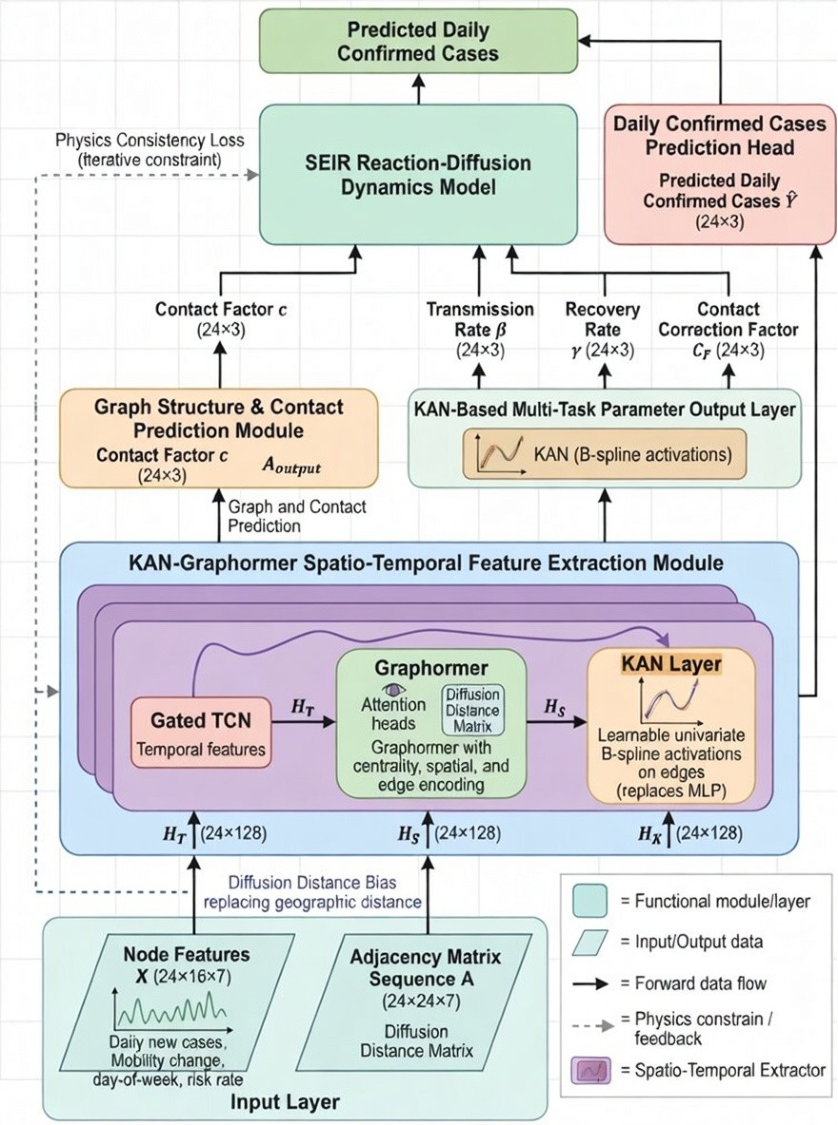
\includegraphics[width=0.8\linewidth]{KAN‑Graphormer混合预测模型总体架构与信息流转图.pdf}
		\caption{Overall architecture of the proposed KAN-Graphormer-SEIR hybrid forecasting framework. The framework consists of four sequential stages: (1) Gated TCN for temporal feature extraction, (2) improved Graphormer for mobility-aware spatial dependency modeling, (3) KAN-based nonlinear decoding, and (4) multi-task output heads for case prediction and epidemiological parameter estimation.}
		\label{fig:2.1}
	\end{figure}
	
	\subsubsection*{Stage 1: Gated Temporal Convolutional Network}
	
	Temporal dependencies were extracted using a Gated Temporal Convolutional Network
	(Gated TCN)~\cite{dauphin2017}. Causal (masked) convolutions preserve temporal
	ordering, and dilated convolutions expand the receptive field exponentially without
	additional parameters. For input $x$ and kernel $f$ of size $K$,
	\begin{align*}
		y_t = \sum_{s=0}^{K-1} f_s \cdot x_{t - d \cdot s}
	\end{align*}
	
	\noindent where $d$ is the dilation factor. Stacking layers with $d = 1, 2, 4, \dots$
	captures both short-term fluctuations and longer-range trends.
	
	Each TCN layer uses a gated activation unit:
	\begin{align*}
		H_t^{(l)}
		= \tanh\!\Bigl(W_1 \star_d H^{(l-1)} + b_1\Bigr)
		\;\odot\;
		\sigma\!\Bigl(W_2 \star_d H^{(l-1)} + b_2\Bigr)
	\end{align*}
	\noindent where $\star_d$ denotes dilated causal convolution, $\odot$ is element-wise
	multiplication, $\tanh(\cdot)$ generates candidate features, and $\sigma(\cdot)$
	acts as a soft gate controlling information flow per channel. The temporal
	representations $H_T \in \mathbb{R}^{B \times N \times H}$ are passed to the spatial
	module; here $B$ is the batch size, $N$ is the number of cities, and $H$ is the hidden dimension.
	
	\subsubsection*{Stage 2: Mobility-Aware Graphormer}
	
	Spatial transmission dependencies were captured by a Graphormer~\cite{ying2021} with
	three mobility-aware encoding mechanisms.
	
	\noindent\textbf{Centrality encoding.}
	Cities with high in-degree and out-degree play distinct roles in disease importation
	and exportation~\cite{kraemer2020}. We inject degree information additively:
	\begin{align*}
		h_i^{(0)} = x_i W_{\mathrm{proj}} + z_{\deg^{-}(v_i)}^{-} + z_{\deg^{+}(v_i)}^{+}
	\end{align*}
	
	\noindent where $x_i \in \mathbb{R}^{F}$ is the input feature vector, $W_{\mathrm{proj}}
	\in \mathbb{R}^{F \times H}$ is a learnable projection, and $z_{\deg^{-}(v_i)}^{-},
	z_{\deg^{+}(v_i)}^{+} \in \mathbb{R}^{H}$ are learnable embeddings for the weighted out-flow strength and in-flow strength computed from the raw (unnormalized) migration intensities $\mathbf{M}(t)$.
	
	\noindent\textbf{Spatial encoding via diffusion distance.}
	The shortest-path encoding of the original Graphormer is replaced by diffusion
	distance. The attention score between cities $i$ and $j$ is
	\begin{align*}
		C_{ij}^{\mathrm{attn}}
		= \frac{(h_i W^Q)(h_j W^K)^\top}{\sqrt{d_k}}
		\;-\; \alpha \cdot d_{\mathrm{diff}}(i,j)
		\;+\; \varepsilon_{ij}(t)
	\end{align*}
	
	\noindent where $W^Q, W^K \in \mathbb{R}^{H \times d_k}$ are query and key projections, $d_k$ is the head dimension, $\alpha > 0$ is a learnable scale and $d_{\mathrm{diff}}(i,j)$ is defined in Eq.~\ref{eq:diffusion_distance}. The diffusion distance term biases attention towards pairs of cities structurally close in
	the mobility network~\cite{coifman2006}.
	
	\noindent\textbf{Dynamic edge encoding.}
	Time-dependent edge weights were incorporated as
	\begin{align*}
		\varepsilon_{ij}(t) = P_{ij}(t) \cdot W^E
	\end{align*}
	\noindent where $P_{ij}(t)$ is the transition probability (Eq.~\ref{eq:mobility_prob})
	and $W^E \in \mathbb{R}$ is a learnable scalar, which enables attention to respond to abrupt mobility changes under interventions~\cite{kraemer2020}.
	
	\noindent\textbf{Gated dense connections.}
	Over-smoothing in deep GNNs~\cite{kipf2017} was mitigated by gated skip connections that blend the current layer with accumulated historical representations:
	\begin{align*}
		H_{\mathrm{in}}^{(l)}
		= g_l \cdot H_{\mathrm{out}}^{(l-1)}
		\;+\; (1 - g_l) \cdot \bar{H}_{D}^{(l)},
		\qquad
		g_l = \sigma(\alpha_l), \;\; \alpha_l \in \mathbb{R}
	\end{align*}
	\noindent where $H_{\mathrm{out}}^{(0)} \equiv h$, $\bar{H}_{D}^{(l)} =
	\frac{1}{l}\sum_{k=0}^{l-1} H_{\mathrm{out}}^{(k)}$ is the dense aggregation of
	all previous outputs, and $g_l$ is a learnable scalar gate initialized to
	$\approx 0.5$. The final spatial representations
	$H_S \in \mathbb{R}^{B \times N \times H}$ encode local epidemic states and
	multi-scale transmission dependencies; the internal structure of a single
	mobility-aware Graphormer layer is summarized in Fig.~\ref{fig:2.3}.
	
	\begin{figure}[H]
		\centering
		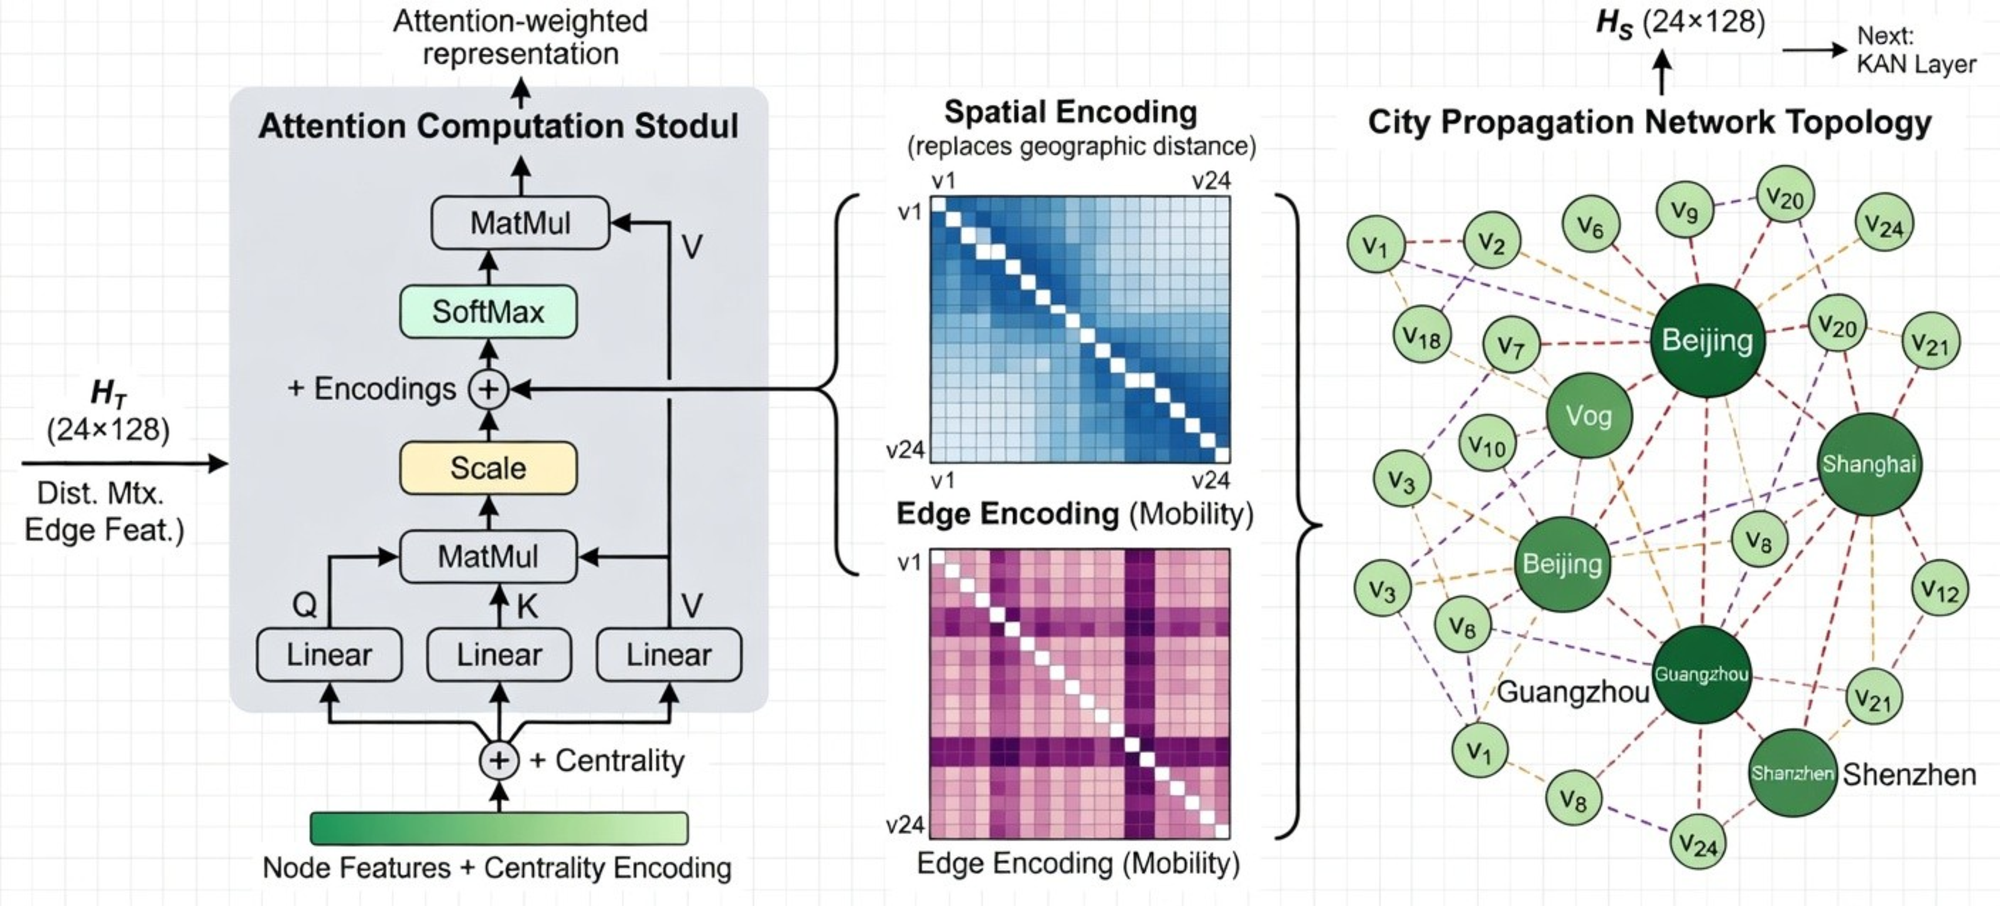
\includegraphics[width=0.7\linewidth]{Graphormer层的内部结构图.pdf}
		\caption{Internal structure of the mobility-aware Graphormer layer.}
		\label{fig:2.3}
	\end{figure}
	
	\subsubsection*{Stage 3: KAN-Based Nonlinear Representation Learning}
	
	We use a Kolmogorov--Arnold Network (KAN)~\cite{liu2025} for nonlinear
	representation learning, motivated by the Kolmogorov--Arnold representation theorem~\cite{kolmogorov1957,arnold1957}:
	\begin{align*}
		f(x_1, \dots, x_n)
		= \sum_{q=1}^{2n+1} \Phi_q\!\left( \sum_{p=1}^{n} \phi_{q,p}(x_p) \right)
	\end{align*}
	
	% Unlike MLPs, which fix activations on nodes, 
	\noindent KAN places learnable
	B-spline activations on edges~\cite{liu2025,deboor1978}:
	\begin{align*}
		\phi(x) = w_b \cdot \mathrm{SiLU}(x) \;+\; w_s \cdot \sum_{i=0}^{G+K-1} \theta_i B_i(x)
	\end{align*}
	\noindent where $\mathrm{SiLU}(x) = x \cdot \sigma(x)$ provides a stable base,
	$B_i(x)$ are B-spline bases of degree $K$ on $G$ intervals, $\theta_i$ are the
	learnable spline coefficients, and $w_b, w_s$ balance the two branches. The local support of B-splines promotes training stability. We use $G = 5$, $K = 3$ with
	$L_2$ regularization on spline coefficients.
	
	\noindent A KAN layer $\Phi : \mathbb{R}^{d_{\mathrm{in}}} \to \mathbb{R}^{d_{\mathrm{out}}}$
	computes each output as a sum of learnable univariate functions (of the
	base-plus-spline form above) over all inputs:
	\begin{align*}
		[\Phi(x)]_o = \sum_{p=1}^{d_{\mathrm{in}}} \phi_{op}(x_p),
		\qquad o = 1, \dots, d_{\mathrm{out}},
	\end{align*}
	where each $\phi_{op}$ carries its own base weight, spline weight, and spline
	coefficients. The $\mathrm{KAN\textrm{--}FFN}$ then stacks two such KAN layers with
	an expansion ratio of $2$, separated by LayerNorm~\cite{ba2016} and Dropout:
	\begin{align*}
		\mathrm{KAN\textrm{--}FFN}(x)
		= \Phi^{(2)}\!\Bigl(
		\mathrm{Dropout}\bigl(\mathrm{LayerNorm}\bigl(\Phi^{(1)}(x)\bigr)\bigr)
		\Bigr),
	\end{align*}
	with $\Phi^{(1)}: \mathbb{R}^{D} \to \mathbb{R}^{2D}$ and
	$\Phi^{(2)}: \mathbb{R}^{2D} \to \mathbb{R}^{D}$. It is integrated within each
	Graphormer layer as:
	\begin{align*}
		H_{\mathrm{out}}^{(l)}
		= \mathrm{LayerNorm}\Bigl(
		H_{\mathrm{attn}}^{(l)} + \mathrm{KAN\textrm{--}FFN}\bigl(H_{\mathrm{attn}}^{(l)}\bigr)
		\Bigr)
	\end{align*}
	
	\noindent The downstream decoder heads are also KAN-based.
	
	\subsubsection*{Stage 4: Multi-Task Epidemiological Decoding}
	
	The latent representation $H_S$ is shared by four output heads.
	
	\noindent\textbf{Incidence forecasting.}
	The model predicts the change relative to the most recent observation (residual
	form), clamped to a feasible range:
	\begin{align*}
		\hat{y}_{i,t+h}
		&= \mathrm{clamp}\bigl( y_{i,t}^{\mathrm{obs}} + \Delta_{i,t+h},\; 0,\; 1.2 \bigr),
		\\[4pt]
		\Delta_{i,\cdot}
		&= W_y^{\mathrm{out}} \, \mathrm{KAN}\bigl(W_y^{\mathrm{in}} h_i + b_y^{\mathrm{in}}\bigr)
		+ b_y^{\mathrm{out}},
		\qquad h = 1, 2, 3
	\end{align*}
	
	\noindent where $h_i \in \mathbb{R}^{H}$ is the latent vector for city $i$,
	$y_{i,t}^{\mathrm{obs}}$ is the last observed normalized case count, and the KAN
	decoder outputs a $T_{\mathrm{out}} \times 3$ residual (3 days $\times$ 3 age groups).
	
	\noindent\textbf{Epidemiological parameter estimation.}
	Three decoder heads estimate the time-varying transmission parameters within
	biologically plausible ranges:
	\begin{align*}
		\beta_{i,t}
		&= \sigma\!\Bigl( \beta_{i,t}^{\mathrm{raw}}
		+ \mathrm{softplus}(\alpha_{\mathrm{reg}}) \cdot r_i \Bigr)
		\times \bigl(\beta_{\max} - \beta_{\min}\bigr) + \beta_{\min},
		\qquad \beta_{i,t}^{\mathrm{raw}} = W_\beta h_i + b_\beta 
		\\[4pt]
		\gamma_{i,t}
		&= \sigma\!\bigl(W_\gamma h_i + b_\gamma\bigr)
		\times \bigl(\gamma_{\max} - \gamma_{\min}\bigr) + \gamma_{\min}
		\\[4pt]
		c_{i,t}^{\mathrm{base}}
		&= \sigma\!\bigl(W_c h_i + b_c\bigr)
		\times \bigl(c_{\max} - c_{\min}\bigr) + c_{\min}
		\\[4pt]
		c_{i,t}^{f}
		&= \exp\!\bigl(-\mathrm{softplus}(\alpha_{\mathrm{lock}}) \cdot L_i(t)\bigr)
		\\[4pt]
		c_{i,t}
		&= c_{i,t}^{\mathrm{base}} \cdot c_{i,t}^{f}
	\end{align*}
	
	\noindent The parameters are constrained to $\beta \in [\beta_{\min}, \beta_{\max}]$
	(with a learnable regional boost $\alpha_{\mathrm{reg}}$ for southern cities,
	$r_i = 1$), $\gamma \in [\gamma_{\min}, \gamma_{\max}]$, and
	$c_{i,t}^{\mathrm{base}} \in [c_{\min}, c_{\max}]$. The base contact factor
	$c_{i,t}^{\mathrm{base}}$ (the ``contact factor $c$'' in Fig.~\ref{fig:2.1}) is
	multiplied by the contact correction factor $c_{i,t}^{f}$ (the ``contact correction
	factor $c_f$'' in Fig.~\ref{fig:2.1}), which reduces effective contact under lockdown,
	where $L_i(t)$ is the city-specific lockdown intensity and $\alpha_{\mathrm{lock}}$ a
	learnable sensitivity. In this study, the bounds were set to
	$\beta_{\min} = 0.1$, $\beta_{\max} = 1.0$, $c_{\min} = 0.1$, $c_{\max} = 1.6$, and
	$\gamma^{-1}_{\min} = 3$, $\gamma^{-1}_{\max} = 7$~days~\cite{tang2020}. These bounds
	span an epidemiologically plausible range for seasonal influenza and serve as weak
	regularizers rather than hard biological constraints under limited observational data.
	
	\subsection*{Physics-Informed Training with Curriculum Learning}
	
	\noindent\textbf{Joint optimization objective.}
	Model training minimizes a composite loss that jointly balances
	data prediction error and violation of epidemiological consistency,
	following the physics-informed neural network (PINN) paradigm~\cite{raissi2019,he2023}:
	\begin{align}
		\mathcal{L}
		=
		\mathcal{L}_{\mathrm{data}}
		\;+\;
		\lambda_1(t) \mathcal{L}_{\mathrm{physics}}
		\;+\;
		\lambda_2 \mathcal{L}_{\mathrm{reg}}
		\label{eq:total_loss}
	\end{align}
	
	\noindent\textbf{Data loss.}
	The prediction loss uses the Huber function~\cite{bishop2006}, which behaves
	quadratically for small residuals (providing smooth gradients near the optimum)
	and linearly for large residuals (limiting the influence of outlier observations
	common in surveillance data):
	\begin{align*}
		\mathcal{L}_{\mathrm{data}}
		= \frac{1}{N T_{\mathrm{out}}}
		\sum_{i=1}^{N} \sum_{h=1}^{T_{\mathrm{out}}}
		\mathcal{H}_{\delta}\!\bigl(y_{i,t+h} - \hat{y}_{i,t+h}\bigr),
	\end{align*}
	
	\noindent\textbf{Regularization.}
	The regularization term combines a spline-coefficient $L_2$ penalty, a
	spline-roughness penalty, and a $R_t$-toward-unity Huber penalty:
	\begin{align*}
		\mathcal{L}_{\mathrm{reg}}
		&=
		\lambda_{\mathrm{spline}}\!\sum_{\theta\in\Theta_{\mathrm{spline}}}\!\|\theta\|_{2}^{2}
		\;+\;
		\lambda_{\mathrm{smooth}}\!\sum_{\theta\in\Theta_{\mathrm{spline}}}\!\|\Delta\theta\|_{2}^{2}
		\;+\;
		\lambda_{R_t}\,\mathcal{H}_{0.5}\!\bigl(R_t^{\mathrm{NGM}},\,1\bigr).
	\end{align*}
	Here $\Delta$ is the first-order difference operator,
	$\|\Delta x\|_2^2 = \sum_j (x_j - x_{j-1})^2$.
	$\Theta_{\mathrm{spline}}$ is the set of all B-spline
	coefficient tensors in the KAN layers, $\mathcal{H}_{0.5}$ is the Huber
	loss with $\delta = 0.5$, and the three terms
	penalize, respectively: spline coefficient magnitude, spline roughness
	(first-order difference), and error of the effective reproduction
	number from unity.
	
	
	\noindent\textbf{Physics loss.}
	To ensure that the predicted incidence trajectories remain consistent with the
	governing SEIR dynamics, the inferred parameters $\beta_i(t)$, $\gamma_i(t)$, and
	$c_i(t)$ are fed into the SEIR ODE system (Eqs.~\ref{eq:metapop_s}--\ref{eq:metapop_r}),
	which is integrated via RK4 to produce an ODE-consistent trajectory $\hat{y}^{\mathrm{ODE}}_{i,t+h}$.
	The physics loss penalizes the discrepancy between this mechanistic trajectory and
	the observed data:
	\begin{align*}
		\mathcal{L}_{\mathrm{physics}}
		=
		\frac{1}{N T_{\mathrm{out}}}
		\sum_{i=1}^{N} \sum_{h=1}^{T_{\mathrm{out}}}
		\mathcal{H}_{\delta}\!\bigl(y_{i,t+h} - \hat{y}^{\mathrm{ODE}}_{i,t+h}\bigr)
	\end{align*}
	
	\noindent A tighter Huber threshold ($\delta = 0.1$) is used for the physics term
	to enforce stricter consistency with the mechanistic model.
	
	\noindent\textbf{Curriculum learning schedule.}
	A critical challenge in physics-informed training is ``regularization dominance,''
	where strong physical constraints applied from the beginning of training prevent
	the network from adequately fitting the data~\cite{wang2021}. To address this, we
	adopted a curriculum learning strategy~\cite{bengio2009} in which the physics
	constraint weight $\lambda_1(t)$ follows a three-phase schedule:
	
	\begin{itemize}
		\item \textbf{Exploration phase} (epochs 0--10): $\lambda_1 = 10^{-6}$.
		The model is nearly unconstrained, learning the dominant statistical
		patterns without strong mechanistic regularization.
		\item \textbf{Integration phase} (epochs 11--30): $\lambda_1$ increases
		linearly from $10^{-6}$ to $10^{-5}$. Physical constraints are
		gradually introduced.
		\item \textbf{Consolidation phase} (epochs 31--150): $\lambda_1 = 10^{-5}$,
		held constant. The curriculum factor and adaptive scaling further
		modulate $\lambda_1$ based on the relative magnitude of data and
		physics losses (see Eq.~\ref{eq:total_loss}).
	\end{itemize}
	
	\noindent This progressive schedule enables the model to first capture the empirical
	structure of the data before being constrained to satisfy mechanistic equations,
	preventing the well-documented failure mode of PINNs under competing
	objectives~\cite{wang2021,raissi2019}.
	
	\noindent\textbf{Training configuration.}
	All models were trained for 150 epochs using the AdamW optimizer with an initial
	learning rate of $10^{-3}$ and a cosine annealing schedule. A batch size of 32
	was used. During physics loss computation, the SEIR ODE was initialized from compartment
	states reconstructed from the incidence series (rather than from the network's
	own predictions), ensuring stable numerical integration during early training. An early
	stopping criterion based on validation loss with a patience of 30 epochs was
	applied to prevent overfitting. All experiments were conducted on a system with
	an NVIDIA GPU and implemented in PyTorch.
	
	\subsection*{Ablation Study Design and Evaluation}
	
	\noindent\textbf{Model variants.}
	Four model variants were constructed by selectively enabling the KAN nonlinear decoder and the physics-informed constraint (Table~\ref{tab:results}). KAN-Graphormer-SEIR enables both. KAN-Graphormer removes the SEIR physics loss while retaining KAN and Graphormer. MLP-Graphormer-SEIR replaces the KAN decoder with a conventional MLP. LSTM~\cite{hochreiter1997} serves as a baseline architecture without explicit epidemiological constraints or KAN-based nonlinear representations.
	
	\noindent\textbf{Data partitioning.}
	The final 20\% of temporally ordered samples was retained as an out-of-time test
	set. Within the preceding 80\% pre-test period, samples were randomly partitioned
	into training (60\% of all samples) and validation (20\% of all samples) subsets.
	This design is described as ``pre-test random train/validation + final temporal
	holdout'' rather than a strict chronological 60/20/20 split.
	
	\noindent\textbf{Fair comparison.}
	To isolate each component's contribution from raw model capacity, all three
	Graphormer-based variants were trained with a hidden dimension of 32 and
	weight decay of $10^{-2}$, so their parameter counts are comparable.%: Full KAN-G (75{,}941) is the largest, followed by NoPhys-KAN-G (60{,}709) and M-Graphormer (59{,}718), whereas the LSTM baseline is much smaller (25{,}993). Any performance or stability difference among the Graphormer-based variants therefore reflects the KAN decoder and the physics-informed constraint rather than model capacity.
	
	\noindent\textbf{Evaluation metrics.}
	Forecasting performance was evaluated using $R^2$, root mean square error (RMSE),
	and mean absolute error (MAE). Epidemiological parameters ($\beta$, $\gamma$, $R_t$) were compared
	against reported ranges for seasonal influenza~\cite{tang2020}. All models were
	trained and evaluated over 20 fixed random seeds, and every reported value is the
	cross-seed mean $\pm$ sem (n=20).
	
	\noindent\textbf{Outbreak probability evaluation.}
	Beyond point forecasting, we estimate the probability of an outbreak event in each city within the forecast horizon. Let $A^{\mathrm{past}}_{i,t} = \frac{1}{7}\sum_{d=0}^{6} y_{i,t-d}$ be the 7-day historical mean incidence and $A^{\mathrm{pred}}_{i,t} = \frac{1}{3}\sum_{h=1}^{3} y_{i,t+h}$ the 3-day predicted mean incidence. With numerical stabilizer $\epsilon = 1$, the relative growth ratio is $g_{i,t} = (A^{\mathrm{pred}}_{i,t} + \epsilon)/(A^{\mathrm{past}}_{i,t} + \epsilon)$. An outbreak event $Y_{i,t} \in \{0,1\}$ is defined by $A^{\mathrm{pred}}_{i,t} \geq y_{\min}$ and $g_{i,t} \geq \rho$, with baseline thresholds $y_{\min} = 30$ and $\rho = 1.25$; robustness is assessed under a lenient $(y_{\min}=20,\ \rho=1.10)$ and a strict $(y_{\min}=50,\ \rho=1.50)$ specification. Future observed cases are used only for offline label construction and never in model inference, preserving temporal causality.
	
	To capture uncertainty from reporting noise and mobility stochasticity, we perform Monte Carlo perturbation inference with $M = 100$ stochastic forward passes. For the $m$-th pass, the normalized input is perturbed as $X_t^{m} = X_t^{\mathrm{in}} + \varepsilon_m$ with $\varepsilon_m \sim \mathcal{N}(0, \eta\,\sigma_{\mathrm{train}}^{2})$, $\eta = 0.05$, and the mobility matrix is frozen at time $t$ and perturbed per horizon as $P_{t+h}^{m} = \mathrm{RowNorm}(P_t + \xi_h^{m})$ with $\xi_h^{m} \sim \mathcal{N}(0, \eta_A\,\sigma_P^{2})$, $\eta_A = 0.05$. Each pass yields predicted incidence $y_{i,t+h}^{m}$ and a corresponding outbreak indicator $Z_{i,t}^{m}$; the outbreak probability is the empirical mean $P_{i,t}^{\mathrm{out}} = \frac{1}{M}\sum_{m=1}^{M} Z_{i,t}^{m}$.
	%, with a Monte Carlo error band P_{i,t}^{\mathrm{out}} \pm 1.96\sqrt{s_{i,t}^{2}/K}$, where $s_{i,t}^{2}$ is the sample variance of $\{Z_{i,t}^{k}\}$ and the variance is bounded by $1/(4K) = 0.0025$.
	
	
	
	
	
	
	
	
	
	
	
	
	
	\section*{Results}
	\subsection*{Ablation Study}
	
	To evaluate the contribution of the KAN decoder and the physics-informed epidemiological constraints, we compared four model variants constructed by selectively enabling each component. The models were trained and evaluated under identical experimental settings to ensure a fair comparison. Table~\ref{tab:results} summarizes the architectural composition of all model variants used in the ablation study.
	
	\begin{table}[H]
		\centering
		\caption{Model variants and forecasting performance evaluated using mean $\pm$ sem (n=20).}
		\label{tab:results}
		\small\setlength{\tabcolsep}{6pt}
		\begin{tabular}{@{}lccccc@{}}
			\toprule
			\textbf{Model} & \textbf{KAN} & \textbf{Physics} & $\boldsymbol{R^2}\uparrow$ & \textbf{RMSE}$\downarrow$ & \textbf{MAE}$\downarrow$ \\
			\midrule
			\textbf{KAN-Graphormer-SEIR} & $\checkmark$ & $\checkmark$ & $\mathbf{0.744 \pm 0.002}$ & $\mathbf{3.503 \pm 0.015}$ & $\mathbf{1.901 \pm 0.012}$ \\
			KAN-Graphormer & $\checkmark$ & --   & $0.743 \pm 0.003$ & $3.511 \pm 0.021$ & $1.907 \pm 0.020$ \\
			MLP-Graphormer-SEIR & --   & $\checkmark$ & $0.743 \pm 0.003$ & $3.510 \pm 0.021$ & $1.896 \pm 0.021$ \\
			LSTM            & --   & --   & $0.737 \pm 0.003$ & $3.547 \pm 0.018$ & $1.962 \pm 0.015$ \\
			\bottomrule
		\end{tabular}
	\end{table}
	
	Table~\ref{tab:results} reports forecasting performance (mean $\pm$ sem) on the held-out test set. The three Graphormer-based variants achieve closely comparable predictive accuracy (mean $R^2$ of $0.743$--$0.744$), indicating that neither the KAN decoder nor the SEIR constraint materially changes point-forecast accuracy. The KAN decoder's contribution is instead training stability: relative to the MLP decoder (MLP-Graphormer-SEIR), the KAN decoder (KAN-Graphormer-SEIR) reduces the cross-seed standard error by roughly one-third on all three metrics ($32\%$ on $R^2$ and RMSE, $44\%$ on MAE) while leaving mean $R^2$ essentially unchanged ($+0.001$). KAN-Graphormer-SEIR consequently attains the lowest cross-seed standard error on every metric---an especially important property in small-sample epidemic forecasting, where estimates from a single random initialization are unstable.
	
	The physics-informed SEIR constraint contributes mechanistic interpretability rather than additional accuracy: it constrains the inferred parameters to remain consistent with SEIR theory and yields interpretable time-varying quantities ($\beta$, $\gamma$, $R_t$; Table~\ref{tab:epi}). The framework thus combines two practical strengths---reproducible cross-seed estimates and epidemiologically meaningful latent parameters---at no cost in predictive accuracy.
	
	
	\begin{table}[H]
		\centering
		\caption{Epidemiological parameters inferred by the physics-enabled models.}
		\label{tab:epi}
		\begin{tabular}{@{}lcc@{}}
			\toprule
			\textbf{Parameter} & \textbf{MLP-Graphormer-SEIR} & \textbf{KAN-Graphormer-SEIR} \\
			\midrule
			$\beta$ (transmission rate, day$^{-1}$) & $0.627 \pm 0.005$ & $\mathbf{0.638 \pm 0.002}$ \\
			$\gamma^{-1}$ (infectious period, days) & $4.17 \pm 0.04$ & $\mathbf{4.20 \pm 0.01}$ \\
			$c$ (contact coefficient) & $0.803 \pm 0.011$ & $\mathbf{0.788 \pm 0.007}$ \\
			$R_t$ (effective reproduction) & $1.955 \pm 0.032$ & $\mathbf{1.969 \pm 0.022}$ \\
			\bottomrule
		\end{tabular}
		
		\vspace{4pt}
		\footnotesize
		Values are mean $\pm$ sem (n=20).
		$\beta$ lies within the prespecified decoder bound $[0.1, 1.0]$ (Methods), and
		$\gamma^{-1}$ lies within the reported seasonal-influenza range
		$[3.0, 7.0]$ days~\cite{tang2020}. The inferred $R_t \approx 2.0$ reflects active
		transmission during the winter influenza season; because the physics term is only
		weakly regularized ($\lambda \sim 10^{-6}$), these parameters are weakly identified
		and should be read as bounded latent summaries rather than independently validated
		biological estimates.
	\end{table}
	
	\begin{figure}[H]
		\centering
		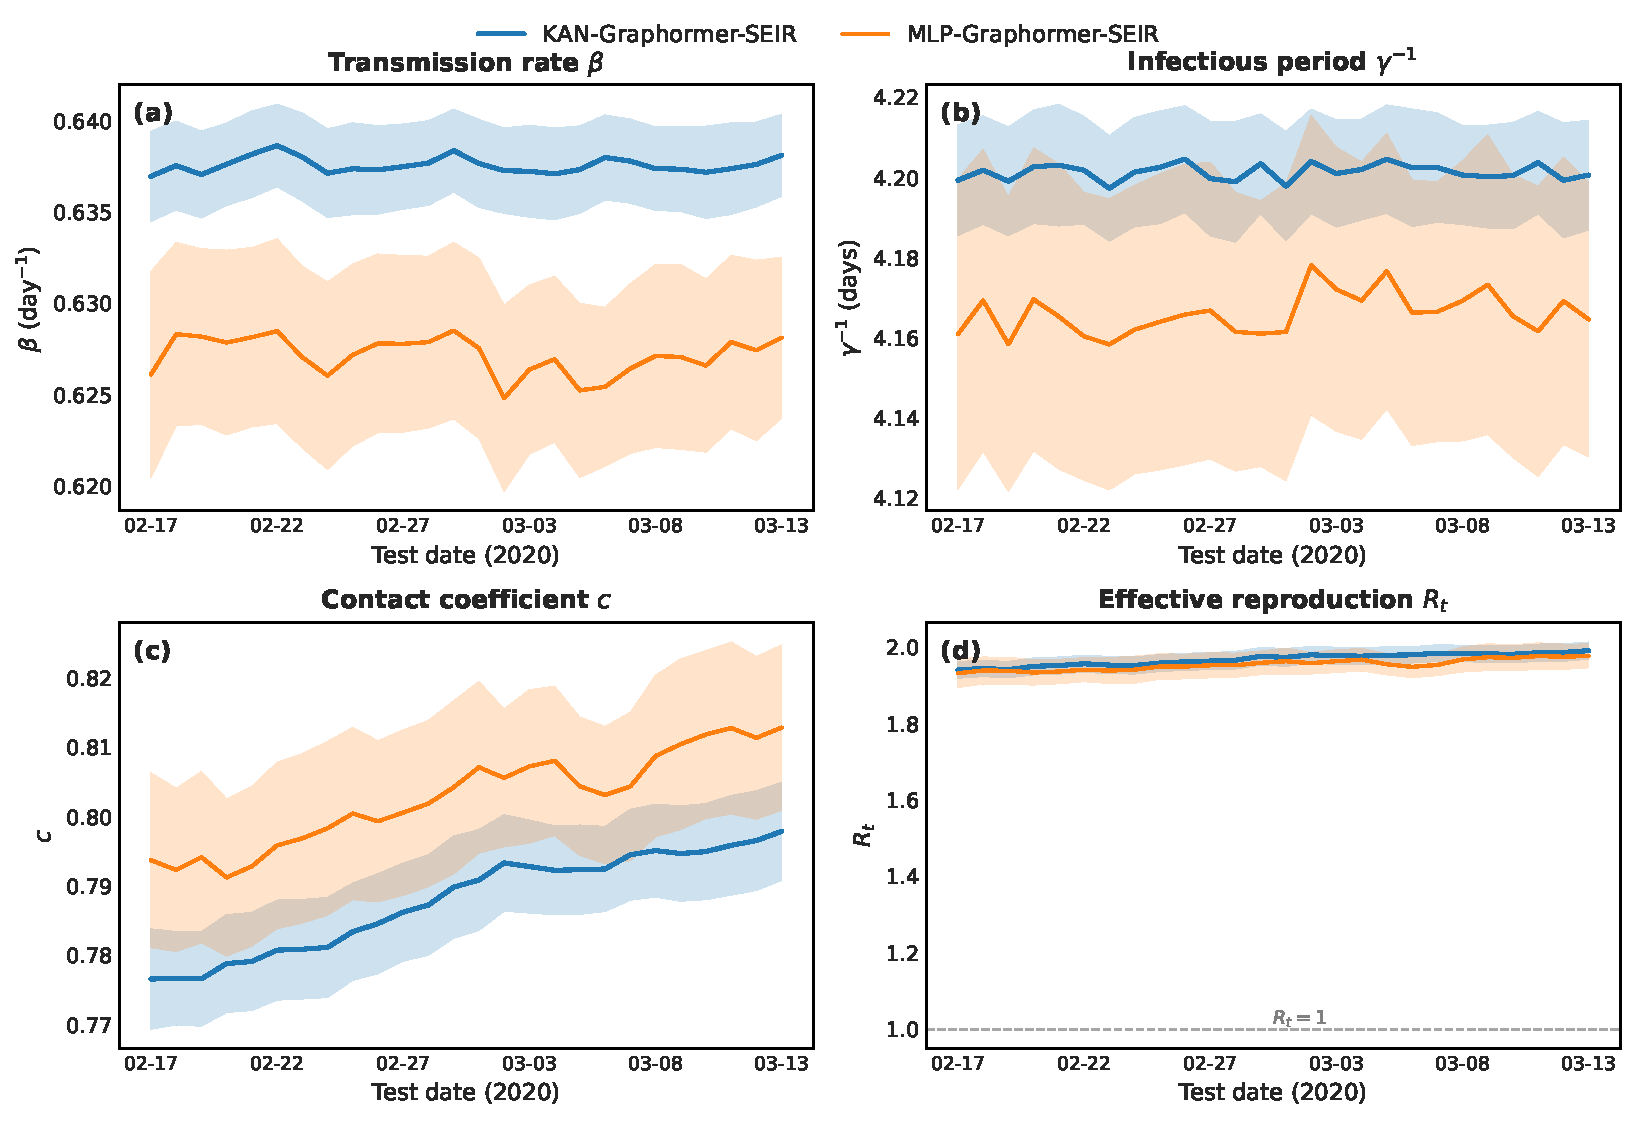
\includegraphics[width=0.92\textwidth]{epi_stability_full_vs_mgraph.pdf}
		\caption{Cross-seed stability of the inferred epidemiological parameters ($\beta$,
			$\gamma^{-1}$, contact coefficient $c$, and $R_t$) for KAN-Graphormer-SEIR (blue) and
			MLP-Graphormer-SEIR (orange) over the 26-day test period. Shaded bands denote $\pm 1$ standard
			error over 20 fixed seeds; the visibly narrower KAN-Graphormer-SEIR bands indicate more
			reproducible parameter estimates across random initializations.}
		\label{fig:epi_stability}
	\end{figure}
	
	Figure~\ref{fig:epi_stability} shows the time-resolved trajectories of the inferred
	parameters together with their cross-seed uncertainty. Across all four parameters the
	KAN-Graphormer-SEIR bands are markedly narrower than those of MLP-Graphormer-SEIR, with the mean
	standard error reduced by a factor of $2.05\times$ ($\beta$), $2.64\times$
	($\gamma^{-1}$), $1.68\times$ ($c$), and $1.45\times$ ($R_t$). This is the
	time-resolved counterpart of the scalar standard errors in Table~\ref{tab:epi} and
	provides direct visual evidence that the physics-informed KAN decoder yields more
	reproducible, better-identified epidemiological parameters across random
	initializations---a property not captured by forecasting accuracy alone. As in
	Table~\ref{tab:epi}, these quantities remain weakly identified latent summaries rather
	than independently validated biological estimates.
	
	\begin{figure}[H]
		\centering
		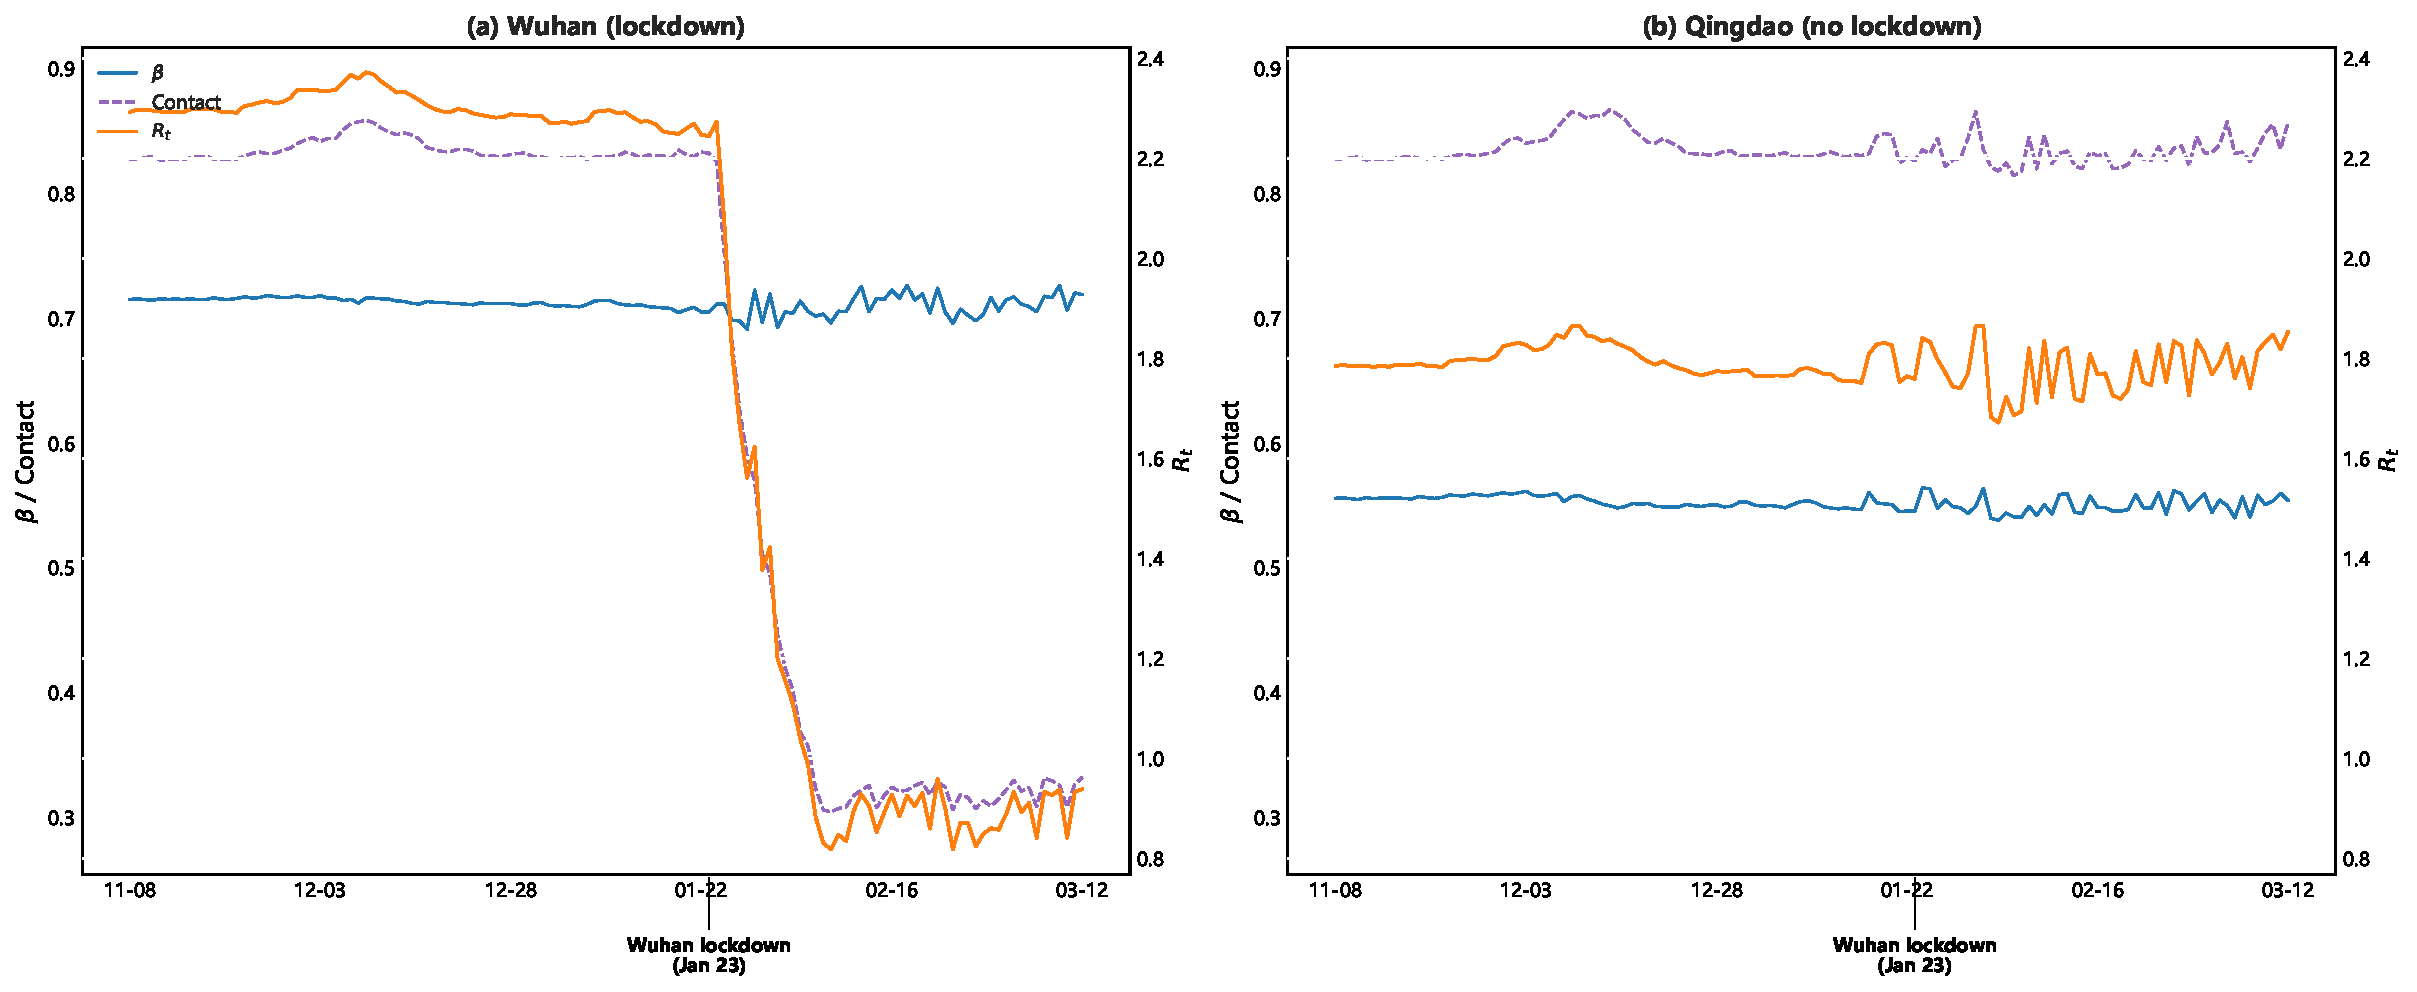
\includegraphics[width=0.80\textwidth]{lockdown_params_comparison.pdf}
		\caption{Model-implied epidemiological latent parameters ($\beta$, contact
			coefficient, and $R_t$) for KAN-Graphormer-SEIR in two representative cities:
			Wuhan (locked down, left) and Qingdao (not locked down, right). The Wuhan lockdown date (January 23, 2020) is marked below the x-axis. These trajectories are descriptive outputs under prespecified parameter bounds and $R_t$ regularization,
			not independently validated parameter ground truth.}
		\label{fig:lockdown}
	\end{figure}
	
	Figure~\ref{fig:lockdown} illustrates these model-implied latent trajectories for two representative cities: in Wuhan (subject to lockdown) the inferred contact coefficient and $R_t$ drop sharply around the January 23, 2020 lockdown, whereas in Qingdao (without lockdown) they remain roughly stable. The quantities reported in Table~\ref{tab:epi} lie within their prespecified decoder bounds ($\beta \in [0.1, 1.0]$, $\gamma^{-1} \in [3, 7]$ days). This agreement is expected because the decoder imposes those bounds. Incidence data alone do not separately identify the transmission-rate and contact multipliers in the present parameterization, and the physics term is only weakly regularized ($\lambda \sim 10^{-6}$); we therefore interpret these trajectories as bounded latent summaries of the fitted model, not as independently validated estimates of biological parameters or causal post-intervention changes.
	
	Together, these findings highlight the importance of integrating data-driven learning with epidemiological knowledge. Rather than functioning solely as a forecasting model, KAN-Graphormer-SEIR serves as an interpretable epidemic intelligence framework capable of simultaneously delivering accurate forecasts, mechanistic insights, and epidemiologically consistent bounded model-implied latent quantities for public health decision support.
	
	
	\subsection*{Forecasting Performance}
	
	
	The forecasting performance of the KAN-Graphormer-SEIR was evaluated on a holdout test set comprising 24 cities% over 26 days 
	using 7-day historical data for the next 3-day prediction. All results are reported in the original case scale after inverse normalization.
	
	As shown in Table~\ref{tab:results}, KAN-Graphormer-SEIR achieved an overall mean $R^2$ of $0.744$ over 20 fixed seeds, indicating that approximately 74.4\% of the variability in
	daily influenza incidence can be explained by the model.
	
	The RMSE ($3.503 \pm 0.015$) and MAE ($1.901 \pm 0.012$) further demonstrate that the prediction errors remain relatively small compared with the observed epidemic magnitude, suggesting satisfactory forecasting precision across different cities.
	
	\begin{figure}[H]
		\centering
		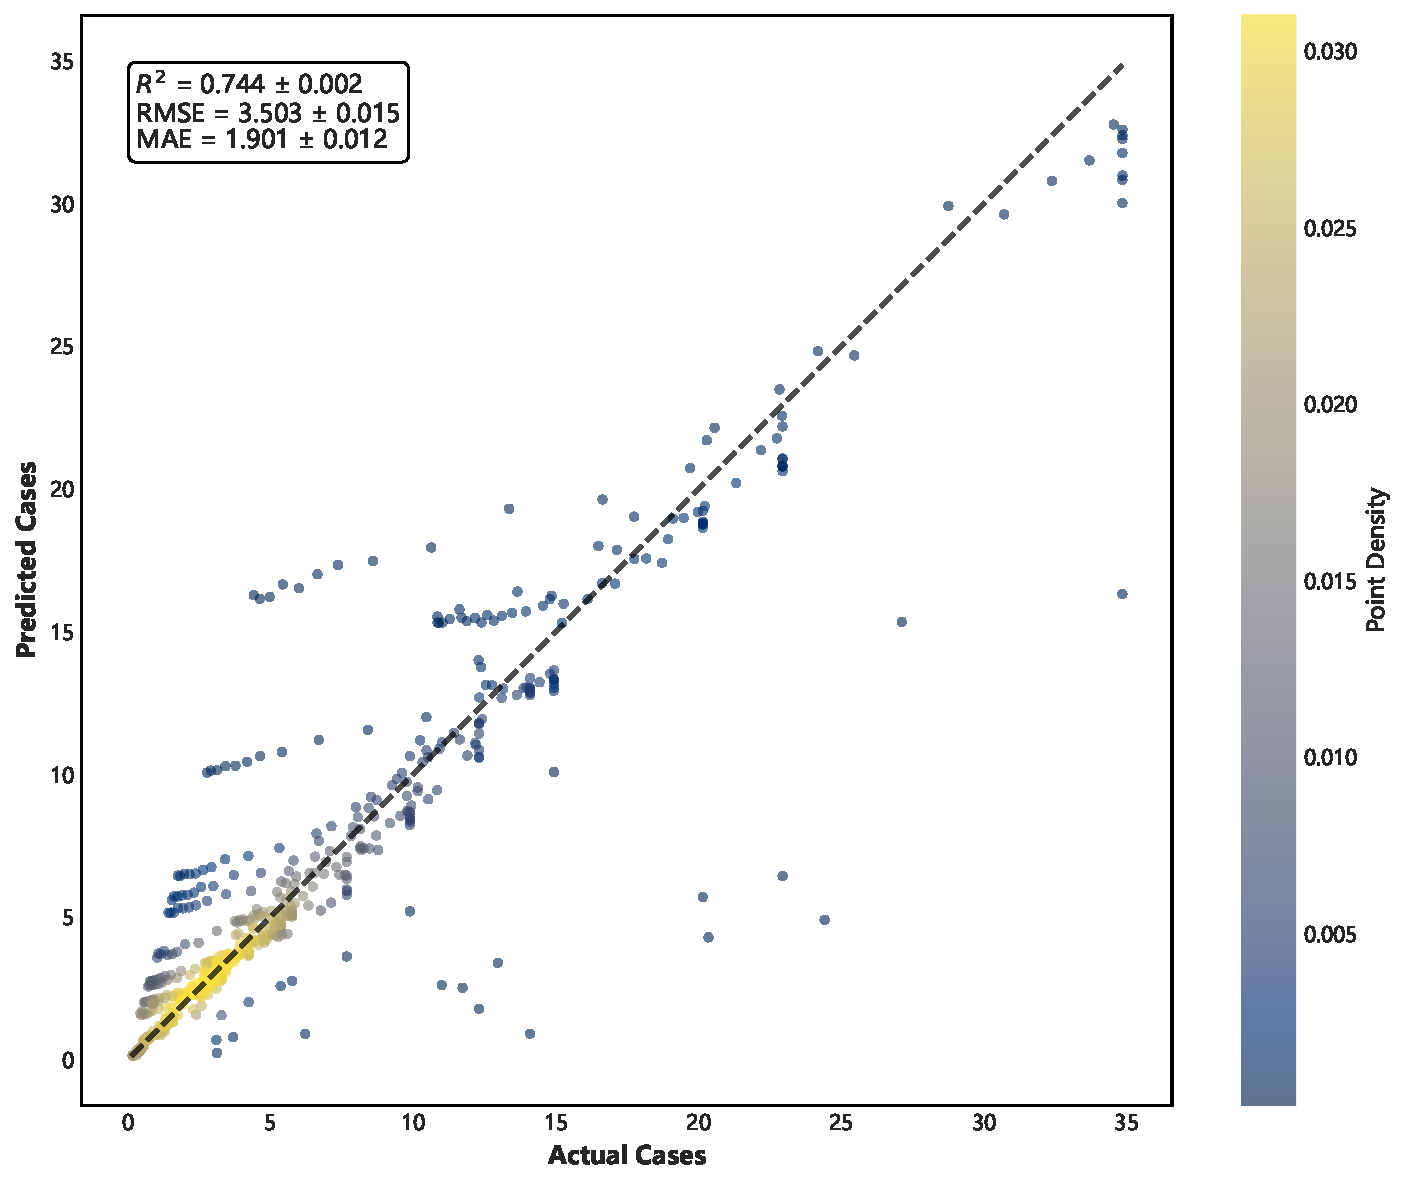
\includegraphics[width=0.6\textwidth]{scatter_Full_KAN_Graphormer.pdf}
		\caption{Predicted vs. observed influenza incidence for the KAN-Graphormer-SEIR model.}
		\label{fig:scatter}
	\end{figure}
	
	Figure~\ref{fig:scatter} illustrates the relationship between predicted and
	observed influenza incidence. Most samples are distributed around the
	45-degree reference line, indicating strong consistency between predictions
	and observations over a wide range of epidemic intensities.
	
	Figure~\ref{fig:city_level} reports $R^2$ (left axis) and RMSE (right axis)
	for each city, ordered by descending $R^2$. Although the overall pooled $R^2$
	is $0.744$ (Table~\ref{tab:results}), per-city performance is highly
	heterogeneous: 11 cities exceed $R^2 = 0.4$, 7 lie between $0$ and $0.4$, and
	6 fall below zero. The two axes are complementary because $R^2$ measures
	relative fit and is independent of case volume, whereas RMSE measures absolute
	error and scales with epidemic magnitude. This distinction is sharpest at the
	extremes: Chongqing attains a satisfactory $R^2$ of $0.51$ yet the largest
	RMSE ($8.8$), whereas Tianjin shows the most negative $R^2$ ($-0.66$) together
	with a small RMSE ($0.70$). The highest relative accuracy is achieved in
	Shenzhen and Guangzhou ($R^2 \approx 0.63$).
	
	The six cities with negative $R^2$ are predominantly low-incidence northern and
	northeastern cities (Tianjin, Qingdao, Jinan, Zhengzhou, Changchun, and Harbin).
	Their near-constant, low-volume case series leave little variance for a relative
	metric to explain, so $R^2$ is unstable there despite small absolute errors; the
	negative values therefore reflect low signal rather than large prediction error.
	However, low $R^2$ is not entirely a small-sample artifact: several
	moderate-to-high-burden cities---most notably Beijing ($R^2 = 0.06$ at $\sim$14.5
	daily cases), along with Hangzhou, Shijiazhuang, and Xi'an---are also poorly
	reproduced, indicating genuine forecasting difficulty in specific metropolitan
	trajectories.
	
	\begin{figure}[H]
		\centering
		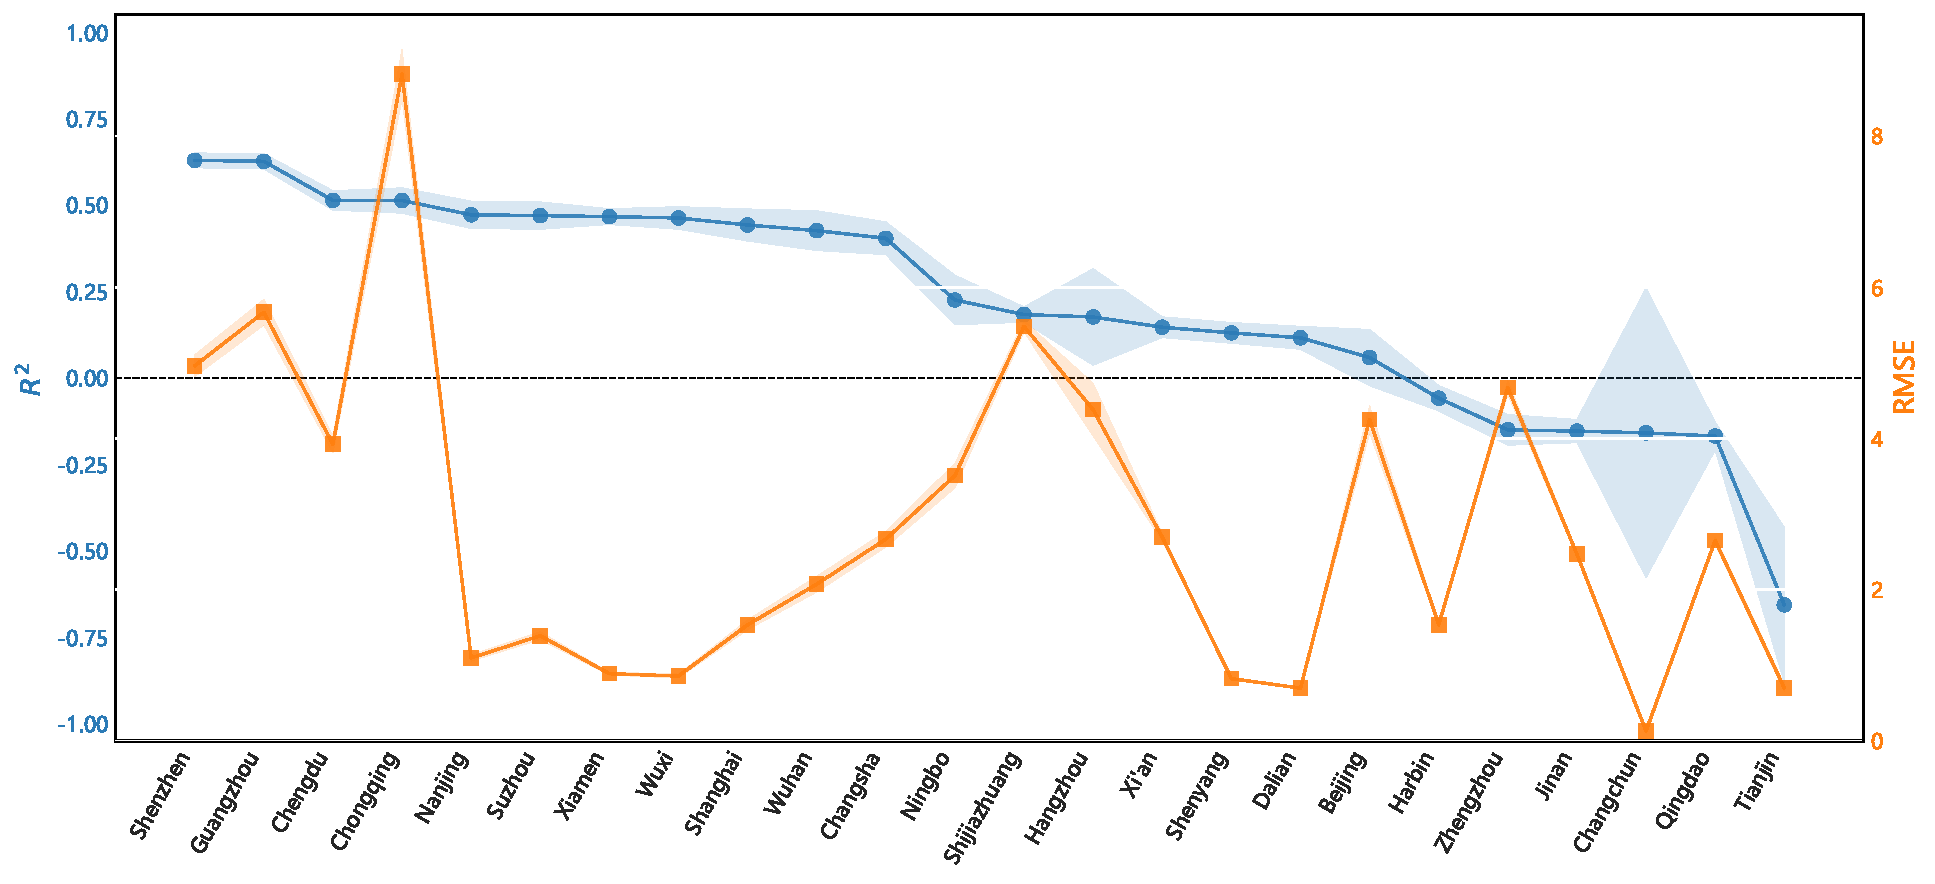
\includegraphics[width=0.85\textwidth]{city_level_Full_KAN_Graphormer.pdf}
		\caption{City-level forecasting performance across 24 cities, showing $R^2$ (left axis) and RMSE (right axis), ordered by descending $R^2$.}
		\label{fig:city_level}
	\end{figure}
	
	\begin{table}[H]
		\centering
		\caption{Forecasting performance stratified by city category.}
		\label{tab:spatial}
		\begin{tabular}{@{}lc@{}}
			\toprule
			\textbf{Subset} & $\boldsymbol{R^2}$ (mean $\pm$ sem) \\
			\midrule
			All cities      & $0.744 \pm 0.002$ \\
			Tier-1 cities   & $0.690 \pm 0.003$ \\
			Tier-2 cities   & $0.728 \pm 0.004$ \\
			\bottomrule
		\end{tabular}
		
		\vspace{4pt}
		\begin{minipage}{0.95\textwidth}
			\footnotesize
			\textit{Note.} Each entry reports the mean $\pm$ sem of the
			pooled $R^2$ across 20 independent training seeds. Within each seed, the $R^2$ for each row is computed from all observations pooled within that row, not by averaging city-specific $R^2$ values. Tier-1 cities are Beijing, Shanghai, Guangzhou, and Shenzhen ($4$ cities); Tier-2 cities are Tianjin, Chongqing, Chengdu, Wuhan, Nanjing, Hangzhou, Xi'an, and Zhengzhou ($8$ cities). The remaining 12 cities are included only in the ``All cities'' row.
			
		\end{minipage}
	\end{table}
	
	Overall, the model demonstrates robust forecasting performance across heterogeneous regions and captures both temporal dynamics and regional variability in influenza transmission.
	
	\subsection*{Epidemiological Dynamics and Parameter Inference}
	
	The KAN-Graphormer-SEIR jointly estimates epidemiological parameters together with case forecasts through a physics-informed SEIR constraint module, enabling interpretable inference of transmission dynamics.
	
	The inferred infectious period ($\gamma^{-1} = 4.2 \pm 0.01$ days) is consistent with reported values for seasonal influenza~\cite{tang2020}. The effective reproduction number averages $R_t \approx 2.0$, indicating active transmission during the winter epidemic peak rather than a declining phase. Because the physics term is weakly regularized and incidence data alone cannot separately identify the transmission-rate and contact multipliers, these parameters should be interpreted as bounded, weakly identified latent summaries.
	
	\begin{figure}[H]
		\centering
		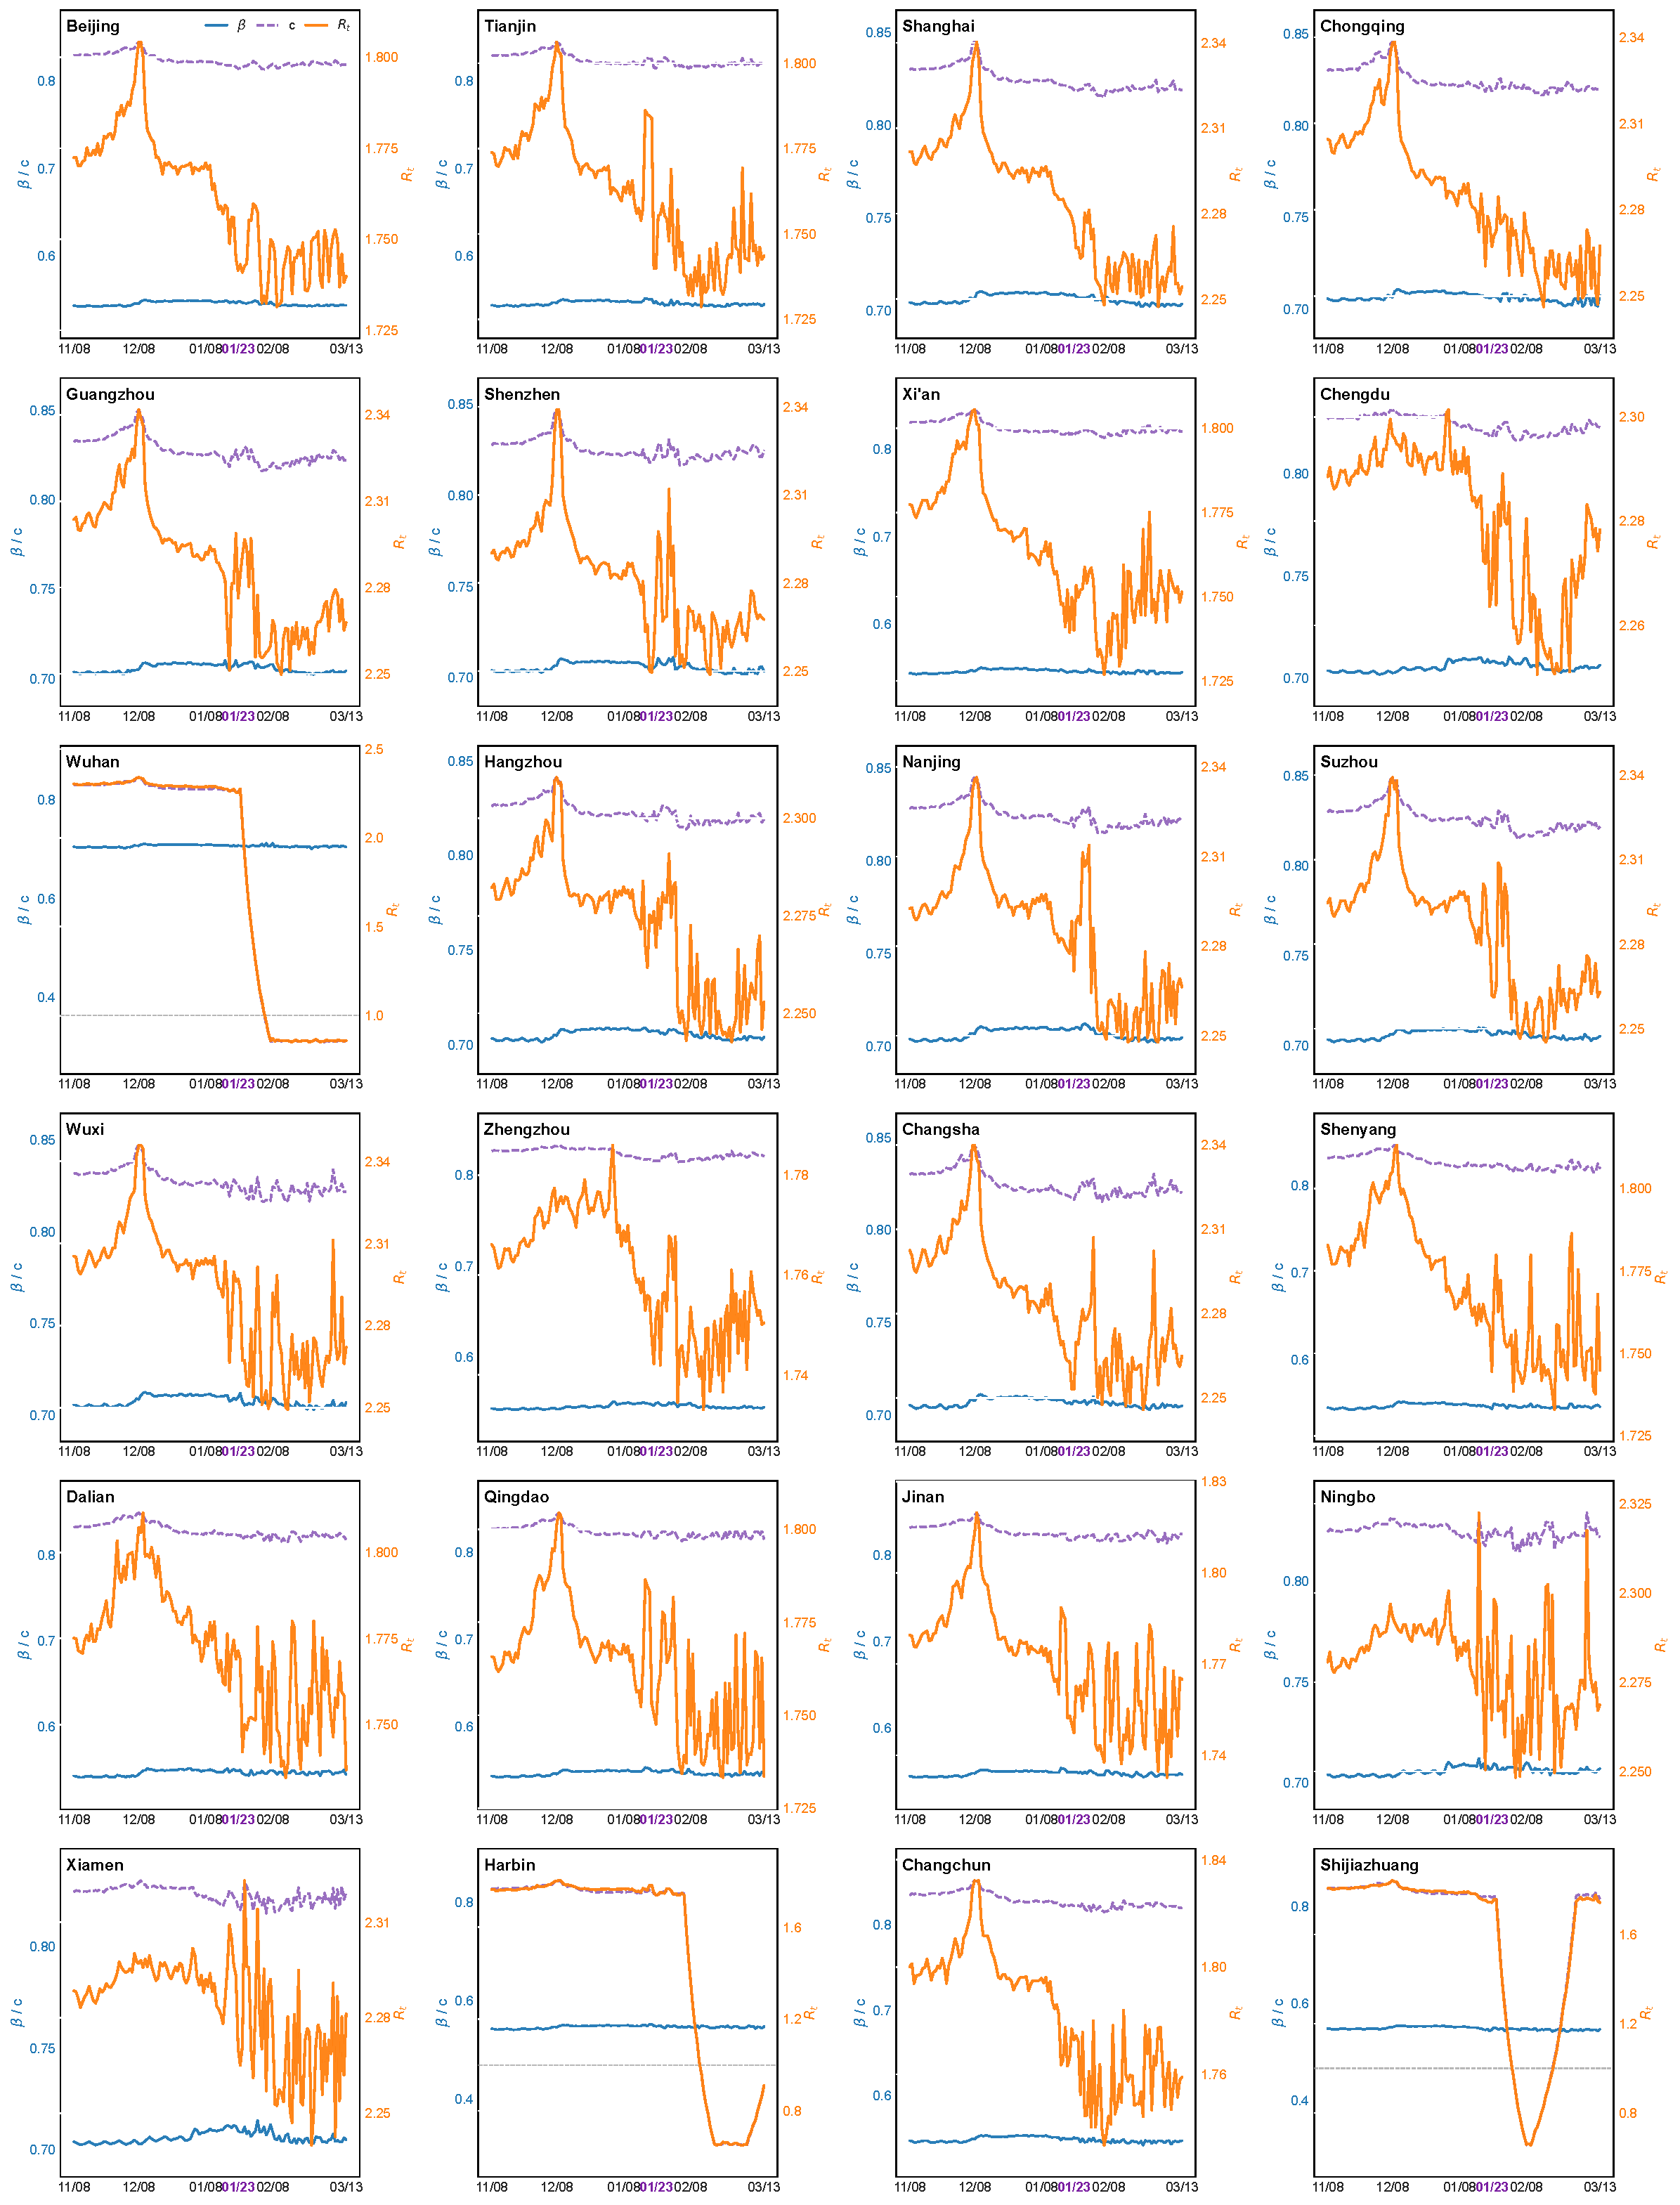
\includegraphics[width=\textwidth]{evolution_24city_grid.pdf}
		\caption{City-specific evolution of inferred epidemiological parameters ($\beta$, contact coefficient $c$, and $R_t$) across 24 cities. The lockdown date (2020-01-23) is marked on the x-axis in purple. Distinct temporal responses among cities reveal substantial spatial heterogeneity in transmission dynamics and intervention effectiveness.}
		\label{fig:evolution}
	\end{figure}
	
	Figure~\ref{fig:evolution} illustrates the temporal evolution of epidemiological parameters for all 24 cities. Several consistent patterns emerge across regions. Following the intervention period, the transmission rate $\beta$ generally decreases or stabilizes, indicating a reduction in effective disease transmission. The contact coefficient $c$ also exhibits declining or flattened trends in most cities, reflecting reduced opportunities for population mixing after intervention measures were introduced. Correspondingly, the effective reproduction number $R_t$ declines below unity in the hardest-hit cities (Wuhan and Harbin) and approaches unity in Shijiazhuang, while remaining elevated in most cities; as $\beta$ and $c$ are only weakly identified from incidence data alone, these trajectories should be interpreted as relative rather than absolute transmission levels.
	
	Despite these common trends, substantial spatial heterogeneity is observed. Major metropolitan areas such as Beijing, Shanghai, Guangzhou, and Shenzhen display relatively stable parameter trajectories, whereas Wuhan, Harbin, and Shijiazhuang exhibit more pronounced fluctuations and stronger post-intervention responses. These differences likely reflect variations in mobility intensity, population density, local intervention timing, and regional epidemic conditions. The results indicate that KAN-Graphormer-SEIR produces city-specific latent trajectories rather than merely fitting aggregate epidemic trends.
	
	The parameter evolution results further suggest that post-intervention changes are spatially heterogeneous. Although most cities exhibit reduced transmission intensity after intervention implementation, the magnitude and timing of these changes vary considerably across regions. These city-specific trajectories show that per-city latent parameters capture localized epidemic responses that a single homogeneous parameterization cannot represent.
	
	
	Taken together, the results indicate that KAN-Graphormer-SEIR performs consistently across three complementary tasks: deterministic case forecasting, exploratory latent-parameter inference, and perturbation-based outbreak sensitivity scoring. The agreement between these evaluation perspectives is consistent with the model capturing both statistical correlations in the data and regionally heterogeneous transmission structure.
	
	\subsection*{Outbreak Risk Forecasting}
	
	Beyond point forecasting, we estimated the probability of an outbreak event in each
	city within the forecast horizon, following the outbreak definition and Monte Carlo
	perturbation inference procedure described in Methods. The outbreak probability
	$P_{i,t}^{\mathrm{out}}$ is the empirical mean of $M = 100$ stochastic forward passes
	under controlled input-feature and mobility-matrix perturbation, with a Monte Carlo
	error band reflecting sampling error only.
	
	Probabilistic outbreak forecasts are generated via Monte Carlo perturbation
	inference. Fig.~\ref{fig:outbreak_merged}
	presents the results for three representative cities---Guangzhou, Wuhan, and
	Shanghai---as three vertically stacked panels (a)--(c). In each panel, daily
	new cases are shown on the left axis (markers), and the outbreak probability
	$P_{i,t}^{\mathrm{out}}$ with its Monte Carlo error band is shown on the right axis. To assess robustness to the detection-threshold specification,
	each panel reports three probability trajectories under a lenient $(y_{\min}=20,\ \rho=1.10)$, a baseline $(y_{\min}=30,\ \rho=1.25)$, and a strict $(y_{\min}=50,\ \rho=1.50)$ threshold.
	
	As shown in Fig.~\ref{fig:outbreak_merged}, the outbreak probability
	trajectories share a consistent rise--peak--decline structure across the
	three cities and across all three thresholds: probability rises as incidence
	increases, peaks during the outbreak window, and declines thereafter. The
	qualitative shape of the risk signal is therefore insensitive to the
	particular threshold, supporting the robustness of the outbreak
	characterization. Shanghai exhibits a sharp, well-defined probability peak
	with narrow Monte Carlo error bands, reflecting relatively low predictive
	uncertainty and a distinct outbreak onset. Wuhan shows a steeper probability
	rise that precedes the case surge---an early warning characteristic---though
	the error band widens during the abrupt lockdown transition, indicating
	elevated uncertainty under regime shifts. Guangzhou maintains sustained
	elevated probabilities throughout a longer outbreak window.
	
	Overall, Monte Carlo perturbation inference transforms deterministic forecasts into perturbation-based risk trajectories, with error bands reflecting Monte Carlo sampling error only.
	The three cities exhibit a shared rise--peak--decline structure in their
	outbreak probability that is preserved across detection thresholds, with
	differences confined to the timing and width of elevated probability
	intervals. This structural consistency across heterogeneous urban
	transmission dynamics and across threshold choices indicates that the
	qualitative outbreak risk assessment is robust and not an artifact of any
	single city's characteristics or of a particular threshold specification,
	supporting its use as a descriptive tool for epidemic situational awareness.
	
	\begin{figure}[H]
		\centering
		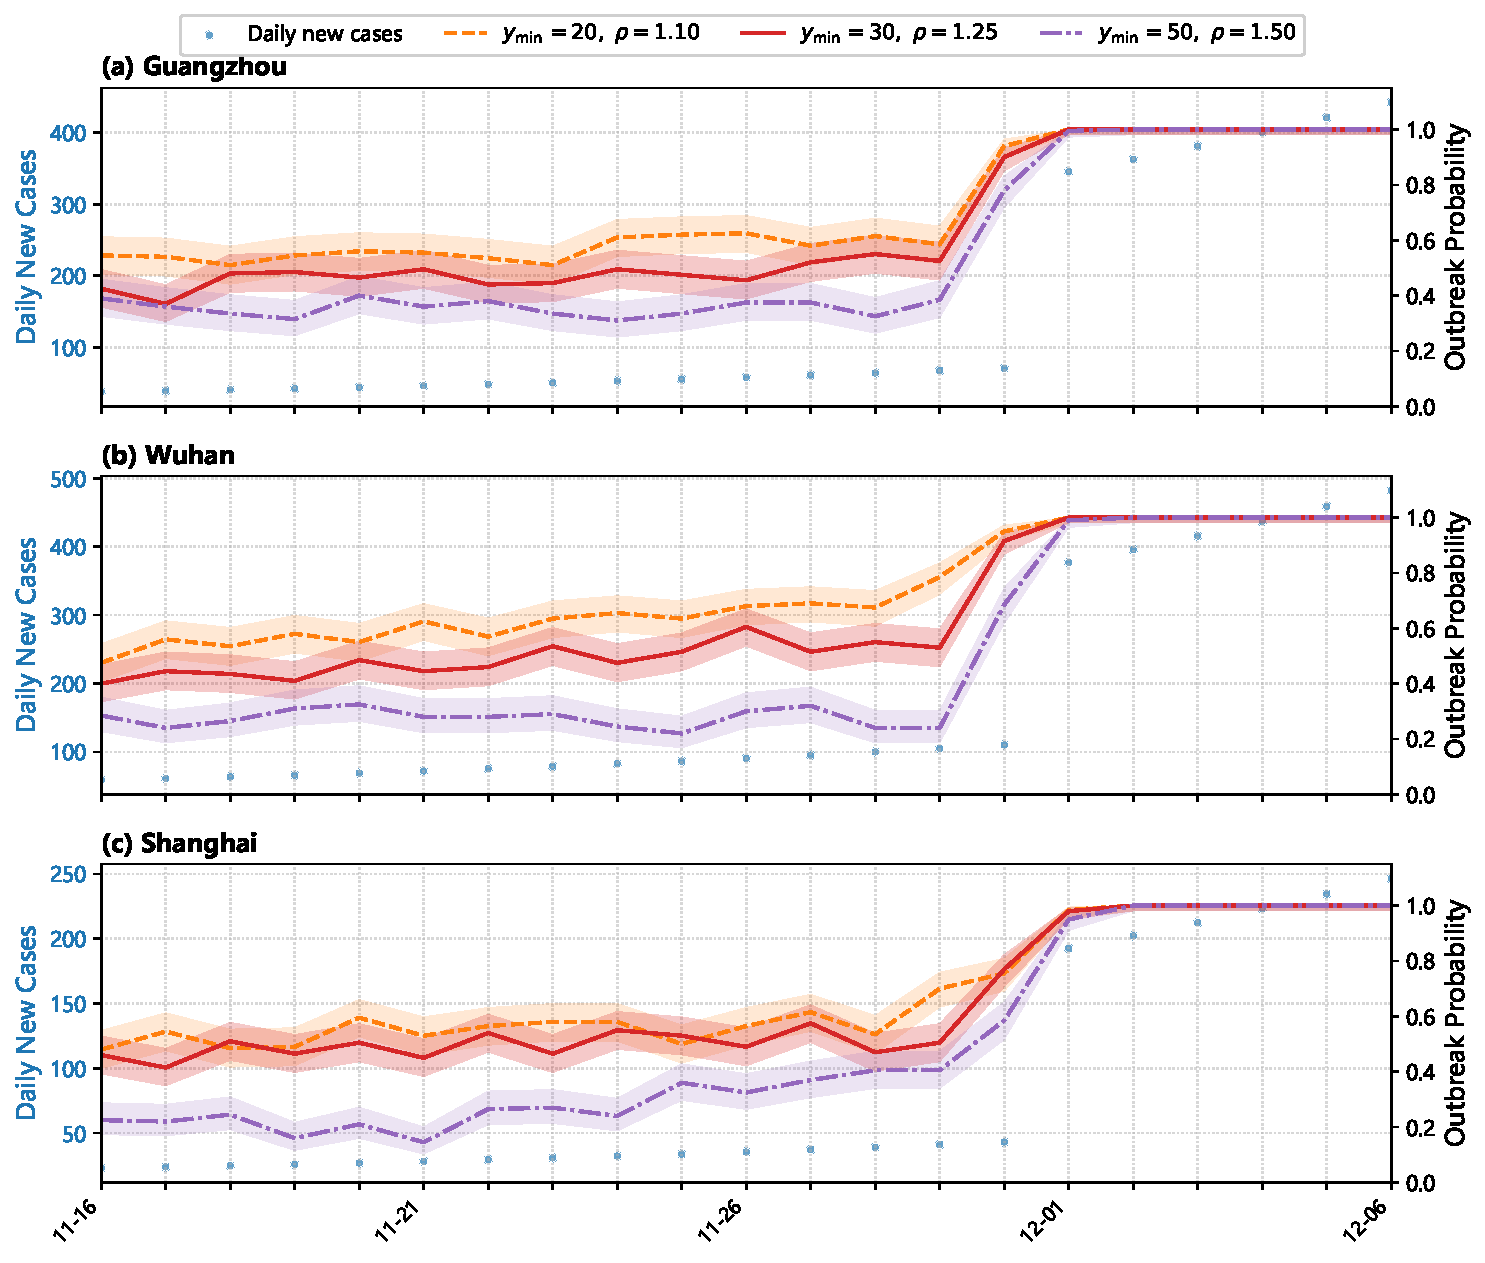
\includegraphics[width=\textwidth]{outbreak_robustness_3panels.pdf}
		\caption{Robustness of outbreak characterization across detection
			thresholds for three representative cities: (a) Guangzhou,
			(b) Wuhan, and (c) Shanghai. In each panel, daily new cases
			(left axis, markers) and the outbreak probability (right axis)
			under a lenient $(y_{\min}=20,\ \rho=1.10)$, baseline
			$(y_{\min}=30,\ \rho=1.25)$, and strict $(y_{\min}=50,\ \rho=1.50)$
			threshold are shown; shaded bands denote Monte Carlo error bands. All three cities and all three thresholds exhibit a
			consistent rise--peak--decline probability structure, indicating
			robustness of the outbreak characterization across heterogeneous
			urban dynamics and threshold choices.}
		\label{fig:outbreak_merged}
	\end{figure}
	
	
	
	
	
	\section*{Conclusion and Discussion}
	
	We proposed \textit{KAN-Graphormer-SEIR}, a physics-informed framework that couples a mobility-aware Graphormer with Kolmogorov--Arnold Network (KAN) layers and an SEIR transmission model. To support this model we reconstructed a daily city-level influenza dataset from province--month surveillance counts and weekly positivity rates via population-weighted PCHIP disaggregation that preserves monthly totals and nonnegativity.
	
	Across 20 fixed seeds on a 136-day, 24-city winter-influenza dataset, the framework attains forecasting accuracy comparable to that of the other Graphormer-based variants ($R^2 \approx 0.744$) while achieving the lowest cross-seed standard error on $R^2$, RMSE, and MAE. The distinguishing contribution of the KAN decoder is therefore not higher mean accuracy but markedly more reproducible estimates: relative to an MLP decoder, it reduces the cross-seed standard error by roughly one-third. The physics-informed SEIR constraint contributes interpretability rather than additional accuracy, yielding bounded, time-varying estimates of $\beta$, $\gamma^{-1}$, $c$, and $R_t$ that fall within seasonal-influenza reference ranges. These two properties---reproducible cross-seed estimates and epidemiologically meaningful latent parameters---are obtained at no measurable cost in predictive accuracy.
	
	Beyond point forecasts, Monte Carlo perturbation inference converts deterministic predictions into outbreak-probability trajectories whose rise--peak--decline structure is robust across detection thresholds and across cities, supporting their use as a descriptive situational-awareness tool.
	
	Several limitations temper these conclusions. First, the daily targets are reconstructed from province--month totals and regional weekly positivity profiles rather than observed city-level daily incidence, so forecasting performance is measured against monthly-anchored proxies; external validation and sensitivity to alternative downscaling schemes are needed. Second, mobility and demographic inputs rely on proxy indicators that may carry measurement bias. Third, the short observation window limits inference of long-term seasonal structure. Fourth, the inferred epidemiological parameters are weakly identified from incidence alone and should be read as bounded latent summaries rather than independently validated biological estimates. Finally, the SEIR formulation omits asymptomatic-transmission heterogeneity and vaccination-induced immunity, and the KAN- and physics-based components increase computational cost relative to simpler baselines.
	
	Future work will extend the framework to multi-year, multi-wave epidemic sequences, improve efficiency through lightweight KAN variants, and pursue stronger interpretability via symbolic regression on the learned activation functions; dynamic mobility prediction and adaptive outbreak thresholds may further improve robustness under abrupt intervention or behavioral shifts. Overall, KAN-Graphormer-SEIR shows that learnable nonlinear decoding and physics-informed constraints together yield a forecasting framework that is simultaneously reproducible, interpretable, and accurate enough for descriptive epidemiological decision support.
	
	
	\section*{Code availability}	
	
	
	
	
	
	
	
	
	
	
	\section*{Acknowledgement}
	C.L. acknowledges financial support from National Natural Science Foundation of China (NSFC, Grant Nos. 12171179). 	
	
	
	
	
	
	
	
	
	
	
	
	\begin{thebibliography}{99}
		
		\bibitem{who2020}
		World Health Organization. Influenza (Seasonal). 
		https://www.who.int/news-room/fact-sheets/detail/influenza-(seasonal)
		
		\bibitem{kermack1927}
		Kermack, W. O. \& McKendrick, A. G. A contribution to the mathematical theory of epidemics. 
		\textit{Proc. R. Soc. A} \textbf{115}, 700–721 (1927).
		
		\bibitem{pastor2015}
		Pastor-Satorras, R. et al. Epidemic processes in networks. 
		\textit{Rev. Mod. Phys.} \textbf{87}, 925–979 (2015).
		
		\bibitem{salathe2010}
		Salathé, M. et al. Human contact networks. 
		\textit{PNAS} \textbf{107}, 22020–22025 (2010).
		
		\bibitem{colizza2008}
		Colizza, V. \& Vespignani, A. Epidemic modeling in metapopulation systems. 
		\textit{J. Theor. Biol.} \textbf{251}, 450–467 (2008).
		
		\bibitem{citron2021}
		Citron, D. T. et al. Comparing metapopulation dynamics of infectious diseases under different mobility models. 
		\textit{PNAS} \textbf{118}, e2007488118 (2021).
		
		\bibitem{feng2018}
		Feng, S. \& Jin, Z. Moment closure of infectious diseases model on heterogeneous metapopulation network. 
		\textit{Adv. Differ. Equ.} (2018).
		
		\bibitem{jia2020}
		Jia, J. S. et al. Population flow drives spatio-temporal distribution of COVID-19 in China. 
		\textit{Nature} \textbf{582}, 389–394 (2020).
		
		\bibitem{zhang2020}
		Zhang, Y., Zhang, A. \& Wang, J. Exploring the roles of high-speed train, air and coach services in the spread of COVID-19 in China. 
		\textit{Transport Policy} \textbf{94}, 34–42 (2020).
		
		\bibitem{murray2003}
		Murray, J. D. \textit{Mathematical Biology II: Spatial Models and Biomedical Applications}. Springer (2003).
		
		\bibitem{gonzalez2008}
		Gonzalez, M. C. et al. Human mobility patterns. 
		\textit{Nature} \textbf{453}, 779–782 (2008).
		
		\bibitem{song2010}
		Song, C. et al. Human mobility scaling laws. 
		\textit{Nat. Phys.} \textbf{6}, 818–823 (2010).
		
		\bibitem{zou2013}
		Zou, J. et al. Influenza in China 2006–2009. 
		\textit{PLoS One} \textbf{8}, e58434 (2013).
		
		\bibitem{yang2018}
		Yang, J. et al. Influenza B epidemiology in China. 
		\textit{Emerg. Infect. Dis.} \textbf{24}, 1536–1540 (2018).
		
		\bibitem{hochreiter1997}
		Hochreiter, S. \& Schmidhuber, J. LSTM. 
		\textit{Neural Comput.} \textbf{9}, 1735–1780 (1997).
		
		\bibitem{wu2020gnn}
		Wu, Z. et al. A comprehensive survey on graph neural networks. 
		\textit{IEEE TNNLS} \textbf{32}, 4–24 (2020).
		
		\bibitem{velickovic2018}
		Veličković, P. et al. Graph attention networks. 
		\textit{ICLR} (2018).
		
		\bibitem{wang2025}
		Wang, X. \& Jin, Z. Spatio-temporal GNN epidemic forecasting. 
		\textit{PLoS Comput. Biol.} \textbf{21}, e1012738 (2025).
		
		\bibitem{gao2021}
		Gao, J. et al. STAN: spatio-temporal attention network. 
		\textit{J. Am. Med. Inform. Assoc.} \textbf{28}, 733–743 (2021).
		
		\bibitem{cao2023}
		Cao, Q. et al. MepoGNN: metapopulation epidemic forecasting. 
		\textit{ECML PKDD} (2023).
		
		\bibitem{mao2024}
		Mao, J. et al. MPSTAN: metapopulation spatio-temporal attention network. 
		\textit{Entropy} \textbf{26}, 278 (2024).
		
		\bibitem{la2021}
		La Gatta, V. et al. Epidemiological neural network with dynamic graph data. 
		\textit{IEEE Trans. Big Data} \textbf{7}, 45–55 (2021).
		
		\bibitem{kapoor2020}
		Kapoor, A. et al. Examining COVID-19 forecasting using spatio-temporal GNNs. 
		\textit{arXiv} (2020).
		
		\bibitem{wu2020}
		Wu, J. T. et al. Nowcasting and forecasting COVID-19 spread in China. 
		\textit{Lancet} \textbf{395}, 689–697 (2020).
		
		\bibitem{raissi2019}
		Raissi, M. et al. Physics-informed neural networks. 
		\textit{J. Comput. Phys.} \textbf{378}, 686–707 (2019).
		
		\bibitem{he2023}
		He, M., Tang, S. \& Xiao, Y. Combining dynamic models and deep neural networks to identify intervention intensity during the COVID-19 pandemic. 
		\textit{PLoS Comput. Biol.} \textbf{19}, e1011535 (2023).
		
		\bibitem{kharazmi2021}
		Kharazmi, E. et al. Physics-informed neural networks for epidemiological models. 
		\textit{Nat. Comput. Sci.} \textbf{1}, 744–753 (2021).
		
		\bibitem{liu2025}
		Liu, Z. et al. KAN: Kolmogorov–Arnold Networks. 
		\textit{ICLR} (2025).
		
		\bibitem{koenig2024}
		Koenig, B. C. et al. KAN-ODEs: Kolmogorov–Arnold network ordinary differential equations. 
		\textit{Comput. Methods Appl. Mech. Eng.} \textbf{424}, 116911 (2024).
		
		\bibitem{guo2025}
		Guo, C. et al. Physics-informed Kolmogorov-Arnold network for fluid mechanics. 
		\textit{Phys. Fluids} \textbf{37} (2025).
		
		\bibitem{ying2021}
		Ying, C. et al. Do Transformers really perform bad for graph representation? 
		\textit{NeurIPS} (2021).
		
		\bibitem{brockmann2013}
		Brockmann, D. \& Helbing, D. The hidden geometry of complex, network-driven contagion phenomena. 
		\textit{Science} \textbf{342}, 1337–1342 (2013).
		
		\bibitem{cdc2020}
		Chinese CDC. Influenza case dataset. https://www.phsciencedata.cn/
		
		\bibitem{cnfi2020}
		Chinese Center for Disease Control and Prevention. Influenza Surveillance Weekly Report. 
		https://ivdc.chinacdc.cn/cnic/
		
		\bibitem{fritsch1980}
		Fritsch, F. N. \& Carlson, R. E. Monotone cubic interpolation. 
		\textit{SIAM J. Numer. Anal.} \textbf{17}, 238–246 (1980).
		
		\bibitem{baidu2020}
		Baidu. Migration scale index dataset. http://qianxi.baidu.com/
		
		\bibitem{stats2020}
		National Bureau of Statistics of China. China Statistical Yearbook (2020).
		
		\bibitem{noaa2020}
		NOAA. Global Surface Summary of the Day. https://www.ncei.noaa.gov/
		
		\bibitem{tianqihoubao}
		Tianqi Houbao. Historical weather data. http://www.tianqihoubao.com/
		
		\bibitem{baiduindex}
		Baidu Index platform. https://index.baidu.com/
		
		\bibitem{lessler2009}
		Lessler, J. et al. Incubation periods of acute respiratory viral infections: a systematic review. 
		\textit{Lancet Infect. Dis.} \textbf{9}, 291–300 (2009).
		
		\bibitem{iuliano2018}
		Iuliano, A. D. et al. Estimates of global seasonal influenza-associated respiratory mortality: a modelling study. 
		\textit{Lancet} \textbf{391}, 1285–1300 (2018).
		
		\bibitem{diekmann2010}
		Diekmann, O. et al. Next-generation matrices for epidemic models. 
		\textit{J. R. Soc. Interface} \textbf{7}, 873–885 (2010).
		
		\bibitem{coifman2006}
		Coifman, R. R. \& Lafon, S. Diffusion maps.
		\textit{Appl. Comput. Harmon. Anal.} \textbf{21}, 5--30 (2006).
		
		\bibitem{dauphin2017}
		Dauphin, Y. N. et al. Gated convolutional networks for language modeling. 
		\textit{ICML} (2017).
		
		\bibitem{kraemer2020}
		Kraemer, M. U. G. et al. The effect of human mobility and control measures on the COVID-19 epidemic in China. 
		\textit{Science} \textbf{368}, 493–497 (2020).
		
		\bibitem{kipf2017}
		Kipf, T. N. \& Welling, M. GCN. 
		\textit{ICLR} (2017).
		
		\bibitem{kolmogorov1957}
		Kolmogorov, A. N. On representation of functions of many variables. 
		\textit{Dokl. Akad. Nauk SSSR} \textbf{114}, 953–956 (1957).
		
		\bibitem{arnold1957}
		Arnold, V. I. On functions of three variables. 
		\textit{Dokl. Akad. Nauk SSSR} \textbf{114}, 5–8 (1957).
		
		\bibitem{deboor1978}
		de Boor, C. \textit{A Practical Guide to Splines}. Springer (1978).
		
		\bibitem{ba2016}
		Ba, J. L., Kiros, J. R. \& Hinton, G. E. Layer normalization. 
		\textit{arXiv} (2016).
		
		\bibitem{tang2020}
		Tang, L. et al. A review of multi-compartment infectious disease models. 
		\textit{Int. Stat. Rev.} \textbf{88}, 462–513 (2020).
		
		\bibitem{bishop2006}
		Bishop, C. M. \textit{Pattern Recognition and Machine Learning}. Springer (2006).
		
		\bibitem{wang2021}
		Wang, S. et al. Physics-informed neural networks optimization issues. 
		\textit{SIAM J. Sci. Comput.} \textbf{43}, A3055–A3081 (2021).
		
		\bibitem{bengio2009}
		Bengio, Y. et al. Curriculum learning. 
		\textit{ICML} (2009).
		
		
		
	\end{thebibliography}
	
	
	
\end{document}

